\documentclass[12pt]{n-te}

\usepackage{dblfloatfix}
\usepackage[pdftitle={Erstsemesterzeitung der Fachgruppe Informatik WS08/09},pdfauthor={Fachgruppe Informatik}]{hyperref}
%\usepackage[latin1]{inputenc}
\usepackage{
  floatflt,
  graphicx,
  ngerman,
  pdfpages,
  subfig,
  subfloat,
  units,
  wasysym
}

\nedition{1}{WS 2008/2009}

%% Trennregeln
\hyphenation{AStA}
\hyphenation{Mit-be-wohnerIn-nen}
\hyphenation{Pro-fessorInnen}
\hyphenation{erwischt}
\hyphenation{viiieel}
\hyphenation{y-Nummer}
\hyphenation{Uniaccount}
%\hbadness=10000

\begin{document}
  \begin{titlepage}
% Der folgende Hack sorgt dafür, dass die Titelseite seitenfüllend eingebunden wird, ohne dass diese zuvor in eine PDF gekapselt werden muss.
\ifpdf
\begin{textblock}{3}(0,0)

\includegraphics[width=\paperwidth]{bilder/titelseite.pdf}
\end{textblock}
\leavevmode\newpage 
%
\includepdf{bilder/titelseite.pdf}
\else

\includegraphics{bilder/titelseite}
\fi
\end{titlepage}


  \setcounter{page}{1}
  \begin{figure*}[t]
    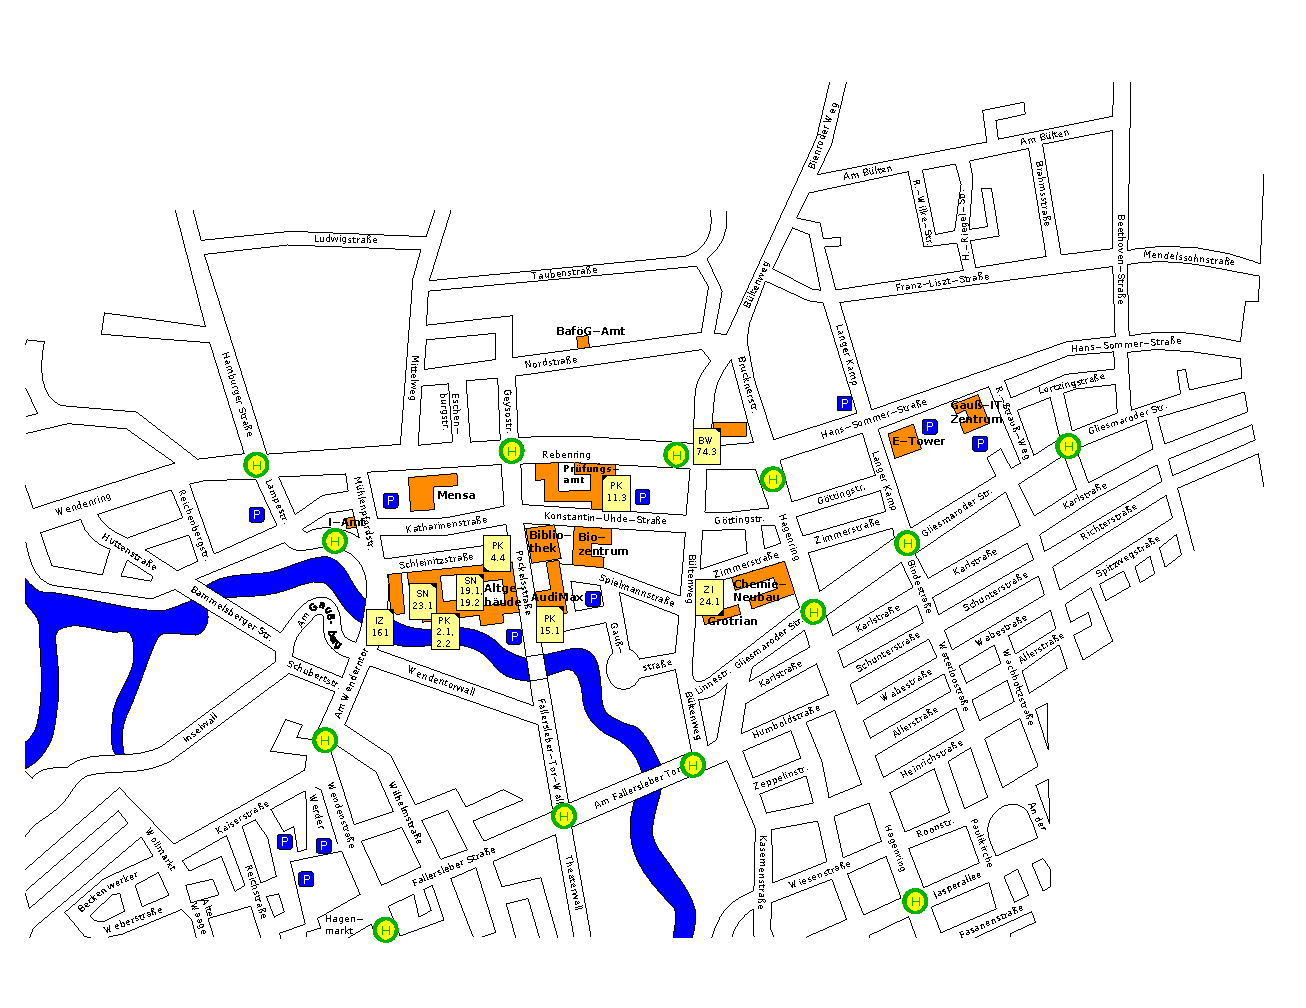
\includegraphics[angle=90]{bilder/plan.pdf}
  \end{figure*}
  \clearpage

  % !TEX root = ../1-te.tex

\section{Vorwort}
\label{vorwort}
	\begin{multicols}{2}
	\subsection*{Willkommen in der Informatik!}	

	Das neue Semester an der TU Braunschweig beginnt und du bist dabei. Die Fachgruppe Informatik (s. Seite \pageref{fachgruppe}) begrüßt dich ganz herzlich an der Uni und möchte dir mit der \enquote{1-ten} den Start vereinfachen. Diese Erstsemesterzeitung der Informatiker soll dir dabei helfen, Antworten auf viele Fragen, die sich zu Beginn des Studiums stellen, zu beantworten.

	\subsubsection*{Aufbau dieses Heftes}
		Der Fokus der ersten Seiten liegt auf den vielen Fragen zum Studienbeginn, deinem Studiengang und der Infrastruktur der Uni. Wir erklären, wie Studienplanung funktioniert und was für Bachelor und Master wichtig ist.
Der Fachgruppenrat Informatik stellt sich vor und beantwortet die Fragen, wer er ist und was er macht.


	\columnbreak

	\begin{center}
		
\includegraphics[width=.7\columnwidth]{bilder/fg-logo/fg-logo.pdf}
	\end{center}

	\subsubsection*{Der Blog}
		Der Fachgruppenrat Informatik betreibt den Blog FGInfo (\fginfoUrl). Dort werden unsere Termine und Veranstaltungen, z.B. Spieleabende, angekündigt und über die hochschulpolitische Arbeit berichtet.
Zusätzlich pflegt die Fachgruppe ein Wiki mit vielen Infos, Tipps und Wissenswertes rund um die Informatik-Studiengänge.
Dieses Heft, die 1-te, gibt es dort auch noch einmal zu finden. Mitunter
ergeben sich noch nach dem Druck Änderungen, gerade bei Terminen, also schau auf jeden Fall dort rein!

	\vspace*{0.5cm}

	Viel Spaß und Erfolg im  Studium wünscht  die\\
	\hspace*{2cm}Fachgruppe Informatik

	\end{multicols}

  \newpage
  \ntoc %% Inhaltsverzeichnis
  \clearpage

  \subsection{Termine}
\label{termine}
Gerade in der Anfangszeit des Studiums gibt es eine Menge zu tun. Damit ihr
nicht das Wichtigste verpasst, haben wir die ersten Termine kompakt f"ur
euch zusammengefasst. Die meisten davon bieten die Gelegenheit Fragen zu
stellen und nebenbei gleich ein paar nette Kommilitonen kennen zu lernen.

Falls ihr es euch nicht schon gedacht habt: Die Spalten B und M geben an,
ob der Termin für Bachelor- oder Masterstudenten gedacht ist. Falls jemand
von euch den eigentlichen Termin verpasst, kann er meist ersatzweise auch
zum anderen erscheinen.

\end{multicols}
\begin{tabular}{|l|l|p{6.7cm}|c|c|c|}
\hline \textbf{Datum} 		& \textbf{Uhrzeit} 	& \textbf{Veranstaltung}						& \textbf{Ort} 	& \textbf{B}	& \textbf{M} 	\\
\hline 26.09. – 30.09.		& 1. Tag: 10:00	 	& Vorkurs Informatik							& PK 2.1		& B				& 				\\
	   17.10. – 21.10.		& 					& 												& 				& 				&    			\\
\hline Mo, 24.10. 			& 09:00 – 10:00		& Begrüßung	durch den Präsidenten				& Stadion		& B				& M				\\ 
\hline 						& 10:00 – 12:00	 	& Infobörse										& Altgebäude	& B				& M				\\
\hline   					& 10:30 – 12:00	 	& Begrüßung (M) \newline durch den Studiendekan	& IZ 160		& 				& M				\\
\hline 						& 13:30 – 15:00	 	& Begrüßung (B) \newline durch den Studiendekan	& PK 11.3		& B				& 				\\
\hline 						& 15:00 – 16:30		& Erste Vorlesung ,,Programmieren 1''			& SN 19.1		& B 			&				\\
\hline Di, 25.10.			& 10:00 – 11:45 	& Erstsemester-Frühstück 						& IZ Plaza 		& B 			& M 			\\ 
\hline 						& 12:00 – 13:30 * 	& FG-Einführung und \newline Stundenplan-Bauen 	& ??? * 		& B 			&  				\\%& ??? * & B &\\
\hline 						& 12:00 – 13:30 * 	& FG-Einführung und \newline Stundenplan-Bauen 	& IZ 160 * 		& 				& M				\\
\hline 						& 13:30 – 15:00 	& Rundgang mit den  Tutorengruppen 				& IZ 160 		& B 			& M				\\
\hline Mi, 26.10.			& 10:00 – 17:00		& Studium Generale								& Altgebäude	& B				& M 			\\
\hline Do, 03.11. 			& 19:00 			& Kneipentour der Fachgruppe 					& IZ 150 		& B 			& M				\\
\hline Mi, 09.11.	 		& 19:00 			& Spieleabend der Fachgruppe 					& vor  150 		& B 			& M				\\
\hline
\end{tabular} 

%%% Local Variables: 
%%% mode: latex
%%% TeX-master: "../../1-te"
%%% End: 

\begin{multicols}{2}

Zum besseren Verständnis der Spalte \textit{Ort} schau in den Abschnitt \textit{Campuskarte} auf Seite \pageref{campuskarte}.

%TODO folgendes muss dann aber auch wirklich umgesetzt werden:
Ihr findet die Termine auch online unter \url{http://fginfo.cs.tu-bs.de/index.php/termine/}.
Falls ihr einen Dienst, ein Handy oder eine Software nutzt, die das iCalender-Format unterstützt
könnt ihr die Termine auch von dort aus einbinden und habt sie somit im Blick. 
Dazu gegören z.B. iPhone, Andoird, Google Calendar, Outlook\ldots Eine Liste 
von ca. 60 Programmen findet ihr unter 
\url{http://en.wikipedia.org/wiki/List_of_applications_with_iCalendar_support}

% TODO es wäre schön, hier zu jedem Termin noch ein oder zwei Sätze zu schreiben, damit man sich darunter etwas vorstellen kann, ähnlich wie bei der TODO-Liste, wo ja auch diverse Textabschnitte folgen.

%In der \textit{Ort}-Spalte stehen meist Raumnummern. F"ur alle R"aume die nicht
%im IZ (steht f"ur Informatikzentrum) liegen, schaut am besten auf den
%Campusplan im Einband. Bei den R"aumen im IZ ist die erste Zahl das Stockwerk, f"ur
%den Rest m"usst ihr dann auf den Plan im Stockwerk schauen (Kleine Falle:
%zwischen EG und 1. OG liegt das Galeriegescho"s - Raum IZ 150 liegt also
%effektiv in der zweiten Etage).
% - Gl"uhweinabend im Informatikzentrum (IZ)

% Dieser Trick hilft uns, eine neue Seite zu erzwingen
% (auf diese passt eh nix sinnvolles mehr) und dennoch die 
% Spaltenlängen auszubalancieren.
\end{multicols}
\newpage
\begin{multicols}{2}


  \section{Gruppen}
\subsection{Fachgruppe bzw. Fachgruppenrat}
\label{fachgruppe}

Die Fachgruppe Informatik besteht eigentlich aus allen 
Informatikstundenten, also ab jetzt auch aus euch. Der Fachgruppenrat 
ist die studentische Vertretung f"ur Studierende der Informatik, also 
eine Art "`Jahrgangssprecher"', die jedes Jahr von euch gew"ahlt werden 
und als Bindeglied zwischen den Studierenden und dem Fachbereich 
fungieren. Oft wird aber auch einfach "`Fachgruppe"' gesagt, wenn man 
eigentlich vom "`Fachgruppenrat"' spricht - vielleicht auch deshalb, 
weil wir keinen großen Wert auf eine Trennung legen, sondern das ganze
eher als Fließenden Übergang zwischen viel und wenig Engagement sehen.

Unsere Hauptaufgabe ist die Vertretung eurer und unserer Meinung 
gegen"uber der Fakult"at in verschiedenen Kommissionen. Kommissionen 
gibt es an der Uni zuhauf, um die verschiedensten Angelegenheiten zu 
regeln. Ein Beispiel ist etwa die Studienkommission, in der ständig 
an den Studienabschl"ussen Bachelor und Master gefeilt wird. Den Bachelor 
gibt es zwar inzwischen schon seit einigen Jahren, aber dank des 
Bildungsstreiks in den Jahren 2009/2010 gibt es nun eine ganze Reihe % TODO mit etwas Glück wird es noch einen Artikel zum Bildungsstreik geben, der dann von hier aus verlinkt werden sollte
von neuen (hoffentlich besseren) Regelungen, die eingearbeitet werden 
müssen.

Zus"atzlich versuchen wir, euch bei Fragen und Problemen rund um das 
Studium weiterzuhelfen. Besonders allen Erstsemestern stehen wir 
gerne mit Rat und Tat zur Seite.  Mehr dazu im Abschnitt ,,Termine'' auf
Seite \pageref{termine}.
%Es gibt zwei Einfühungstermine, an denen wir euch einiges rund um die 
%Uni erz"ahlen m"ochten: ??????

\subsubsection*{FG-Blog}

Auf unserer Webseite \url{http://fginfo.cs.tu-bs.de} seht ihr nicht 
nur, welche Schwerpunkte wir gerade bei unserer Fachgruppenarbeit setzen, 
sonder ihr werdet auch "uber aktuelle Veranstaltungen informiert, und k"onnt 
die Erstsemesterzeitung (die ihr gerade in Händen haltet), herunterladen. 
Am besten abonniert ihr unseren RSS-Feed, dann bekommt ihr automatisch 
mit, wenn es etwas neues gibt.

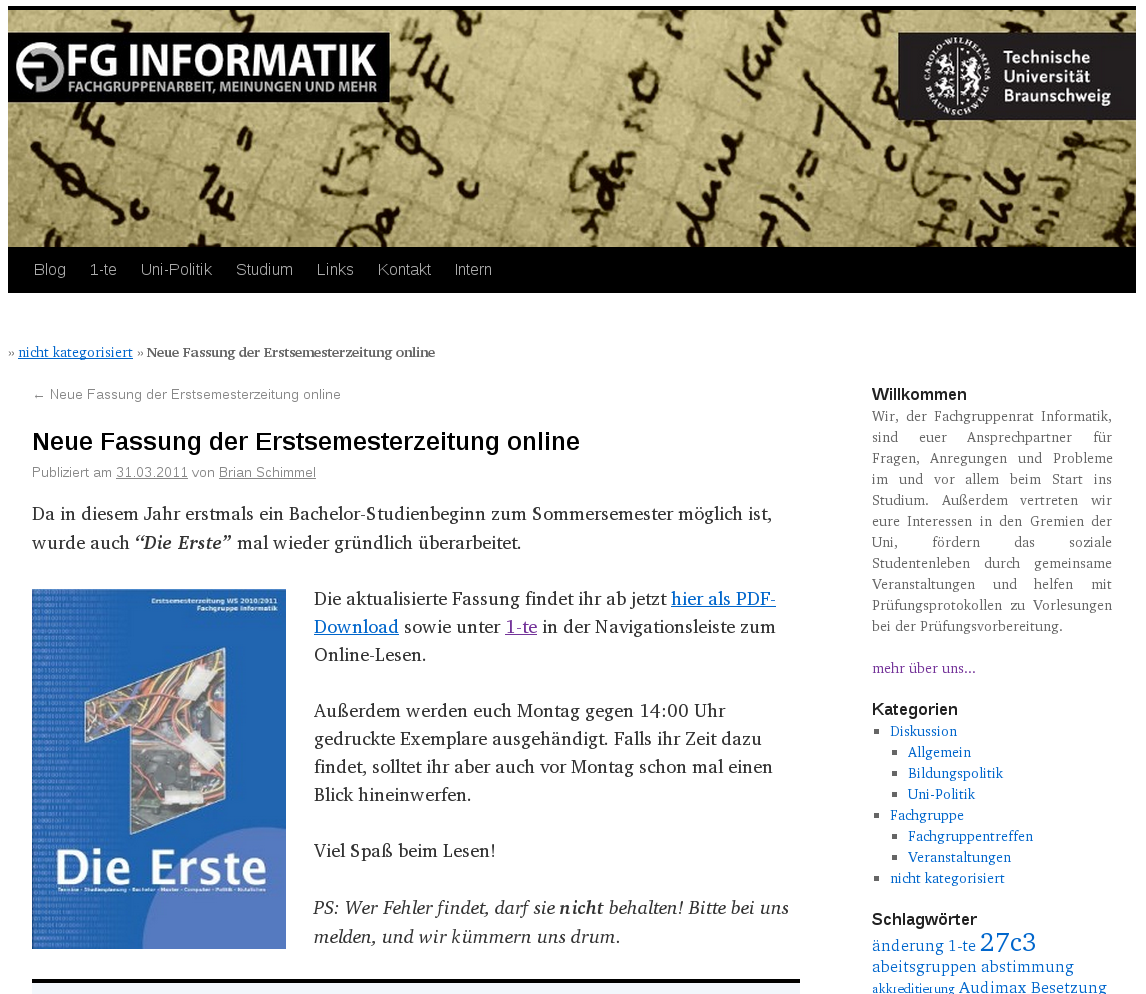
\includegraphics[width=\columnwidth]{bilder/fgblog.png}

Wenn ihr uns persönlich Fragen ansprechen wollt, kommt 
in unsere regelmäßige Sprechstunde, oder zum wöchentlichen Fachgruppentreffen.
Die konkreten Termine standen bei Drucklegung noch nicht fest, aber ihr könnt
sie auf unserem oben genannten Blog nachlesen. Wir haben praktisch immer wichtige 
Neuerungen zu diskutieren und suchen permanent Unterstützung und 
Nachwuchs. Ab und zu beim Fachgruppentreffen herein zu schauen ist 
nicht nur der perfekte Einstieg, um sich selbst einmal einzubringen, 
sondern gibt euch euch die Möglichkeit, immer auf dem neuesten Stand 
der Entwicklungen zu bleiben, die euch letztlich selbst betreffen werden.

\subsection{Tutorien}

% TODO Der Begriff Tutorium ist hier recht eigenwillig genutzt. An den meisten anderen Unis versteht man unter "Tutorium" eher das, was hier "Praktikum" oder "Übung" ist, und dort ist dann "Praktikum" wieder was ganz anderes. Darauf könnte man kurz hinweisen.

% TODO dieser Abschnitt ist aus diverse Kapiteln zusammengeklebt und braucht dringend noch Aufräumung!

In diesem Abschnitt geht es um eure Tutorengruppen, die aus 2 Tutorengruppenleitern (Tutoren) sowie 10--15 Erstis bestehen und euch den Einstieg ins Studium erleichtern sollen.\\
Erfahrungsgem"a"s treten in der Anfangszeit einige Fragen auf. Oft wei"s man noch nicht genau, an wen man sich wenden sollte oder kann den etwas bescheidenen Internetseiten der TU nicht die richtigen Informationen entlocken. In diesen F"allen sind die Tutoren die richtigen Ansprechpartner.\\

% TODO hier zerbricht die schöne neue Ordnung - gehört der Folgende Absatz nach "Fachgruppe" oder nach "Erste Tage"?
Vom besonderen Interesse dürften dabei die allgemeine Einführung sein,
sowie das Ersti-Begrüßung mit anschließenden Rundgang mit der
Tutorengruppe.
Dazu werden wir euch nach dem Frühstück studentischen 
Tutoren zuteilen, mit denen ihr das Unigel"ande und Anderes erkunden 
k"onnt. Bei ihnen k"onnt ihr auch die ersten Fragen loswerden, wenn 
ihr nicht bei einem der beiden Beratungstermine davor wart.
Die Einteilung findet nach dem Frühstück statt und erfolgt nach
Bachelor und Master getrennt.
Jedem Ersti soll in der Einf"uhrungswoche (s. Termine) eine Tutorengruppe zugeteilt werden. Damit auch ihr wisst, an wen ihr euch wenden k"onnt, solltet ihr diese Einteilung und das anschlie"sende erste Treffen nicht verpassen!\\
Dort habt ihr dann die M"oglichkeit in "uberschaubarer Runde andere Informatikstudenten des 1. Semesters kennen zu lernen, Fragen zu stellen, weitere Informationen zu euren Veranstaltungen und Dozenten zu erhalten und das Campusgel"ande kennen zu lernen.\\
Scheut euch nicht einen der Tutoren zu kontaktieren. Ihr k"onnt euch auch nachtr"aglich noch in eine Tutorengruppe einteilen lassen, da weitere Treffen geplant sind. Dazu schreibt bitte eine Mail an die Fachgruppe \nurl{fginfo@tu-bs.de} oder direkt an einen der Tutoren.\\
Damit ihr auch ein paar Gesichter zuordnen k"onnt - gerade wenn ihr eventuell selbst noch keinen Tutor habt - sind hier Fotos einiger Tutoren abgebildet:

% TODO hier evtl. den Unterschied zwischen Tutor und Mentor erwähnen?

\end{multicols}

% TODO Bilder aktualisieren, angeben, ob der jenige Bachelors oder Masters betreut (ist ja nicht immer identisch damit, was man selbst gerade ist)

\paragraph{Bachelor} \ \\

\npicture[0.3\linewidth]
{bilder/tutoren/kris.jpg}
{Christoph\\ 3. Semester Master\\ admin@keeg.de}
\hfill
\npicture[0.3\linewidth]
{bilder/tutoren/dominik.png}
{Dominik\\1. Semester Master\\ d.schuermann@tu-bs.de}
\hfill
\npicture[0.3\linewidth]
{bilder/tutoren/franziska.jpg}
{Franziska\\5. Semester Bachelor\\ f.werk@tu-bs.de}
\par \ \par
\npicture[0.3\linewidth]
{bilder/tutoren/hella.png}
{Hella\\ 1. Semester Master\\ h-f.hoffmann@tu-bs.de}
\hfill
\npicture[0.3\linewidth]
{bilder/tutoren/johannes.png}
{Johannes\\ 5. Semester Bachelor\\ J.Starosta@tu-bs.de}
%\hfill
%\npicture[0.3\linewidth]
%{bilder/tutoren/}
%{Judith\\ 5. Semester Bachelor\\ judith.hilpert@web.de}
\hfill
\npicture[0.3\linewidth]
{bilder/tutoren/marekd.jpg}
{Marek\\ 1. Semester Master\\ m.drogon@tu-bs.de}
%\hfill
%\npicture[0.3\linewidth]%{}
%{bilder/tutoren/}
%{Christina\\ 5. Semester Bachelor\\c.eberth@tu-bs.de }
%\hfill
%\npicture[0.3\linewidth]%{}
%{bilder/tutoren/}
%{Christoph\\ 5. Semester Bachelor\\ christoph.harburg@web.de }
\par \ \par

%\npicture[0.3\linewidth]%{}
%{bilder/tutoren/}
%{Serj\\ 1. Semester Master\\s.dechand@tu-bs.de }
%\hfill
%\npicture[0.3\linewidth]%{}
%{bilder/tutoren/}
%{Jonathan\\ 5. Semester Bachelor\\ j.koscielny@tu-bs.de}%.eberth@tu-bs.de }
%\hfill
%\npicture[0.3\linewidth]
%{bilder/tutoren/olav.jpg}
%{Olav\\ 3. Semester Master\\ olav\_bk@web.de}
%\hfill
\npicture[0.3\linewidth]
{bilder/tutoren/sebastian.jpeg}
{Sebastian\\ 1. Semester Master\\ se.busse@tu-bs.de}
\par \ \par

\paragraph{Master} \ \\
\npicture[0.3\linewidth]
{bilder/tutoren/martinw.jpg}
{Martin\\ 3. Semester Master\\ m.wegner@tu-bs.de}
\hfill
\npicture[0.3\linewidth]
{bilder/tutoren/henning.png}
{Henning\\ 4. Semester Master\\ h.guenther@tu-bs.de}
\hfill
\npicture[0.3\linewidth]
{bilder/tutoren/jan.jpg}
{Jan\\ 3. Semester Master\\ jhkluth@gmx.de}
\par \ \par
\npicture[0.3\linewidth]
{bilder/tutoren/brian.jpg}
{Brian\\ 3. Semester Master\\ b.schimmel@tu-bs.de}
\hfill
%\npicture[0.3\linewidth]
%{bilder/tutoren/stephan.jpg}%Christopher Lössl < c.loessl@tu-bs.de>
%{n\\ Christopher 2. Semester Master\\ c.loessl@tu-bs.de}
%\npicture[0.3\linewidth]
%{bilder/tutoren/stephan.jpg}
%{Stephan\\ 5. Semester Master\\ stephan.friedrichs@tu-bs.de}

\begin{multicols}{2}
%%% Local Variables: 
%%% mode: latex
%%% TeX-master: "../../1-te"
%%% End: 

\subsection{Hochschulpolitik -- Einmischen an der Universität}

Auch wenn ihr jetzt erst ein Studium aufgenommen habt, habt ihr sicherlich 
schon mitbekommen, dass an der TU nicht immer alles rund läuft.

Was vermutlich nur die Wenigsten wissen: Auch als Studierende kann man sich 
dafür einsetzen, dass sich etwas ändert. So gibt es für nahezu alle Belange Gremien 
an der Uni, wo auch fast immer Studierende mitmachen, oft sogar mit Stimmrecht. 
Obwohl wir Studierenden die größte Gruppe der Uni sind, haben wir dabei aber nahezu immer 
weniger Stimmen als die Professor/innen oder Mitarbeiter/innen. 

Trotzdem lässt sich vieles erreichen. Wer mitmachen möchte, kann einfach 
mal zu einen unserer Fachgruppentreffen kommen. Der aktuelle Termin steht immer 
 auf unserer Webseite \fginfoUrl.

Im folgenden stellen wir euch einmal alle Gremien vor.
Auf der vorherigen Seite findet ihr eine grafische Übersicht über die verschiedenen Gremien. Sie sind dort hierarchisch geordnet.

\subsubsection*{Organe der Studierendenschaft}

Die Studierendenschaft besteht aus allen Studierenden der TU Braunschweig, also auch dir!
Man wird mit der Einschreibung automatisch Mitglied. Dazu gehört auch ein Semesterbeitrag, den jede/r 
zusätzlich zu den Studiengebühren zahlt und womit die Studierendenschaft ihre Aufgaben finanziert. 
Dazu gehören neben dem Semesterticket, dem Hilfsfond für Studierende in Not und der 
Fahrradwerkstatt vor allem die Aufgaben der Fachgruppen, Fachschaften und des AStA. Auch diese
Erstizeitung wurde darüber finanziert.
\\
\\
Die Studierendenschaft gliedert sich wiederum in Fachschaften und Fachgruppen.
Alle Studierenden einer Fakultät bilden zusammen die \textbf{Fachschaft (FS)}, davon gibt es derzeit insgesamt sechs.
Diese werden wiederum in  \textbf{Fachgruppen (FG)} aufgeteilt. Alle Studierenden eines Studienfaches bilden eine Fachgruppe, 
somit besteht die Fachschaft unserer Fakultät aus den Fachgruppen Informatik, Mathematik, Medienwissenschaften, Sozialwissenschaften sowie 
Wirtschaftsinformatik. Die Studierenden einer Fachschaft werden  durch den 
\textbf{Fachschaftsrat (FSR)} vertreten. Da wir viele verschiedene Fächer haben, wichtige Dinge aber oft gemeinsam besprochen werden müssen,
trifft sich bei uns der Fachschaftsrat üblicherweise einmal pro Monat. 
Bei wichtigen Dingen (üblicherweise wenn unerwartet ein bestimmtes Gremium einberufen wird) kann dies auch öfters passieren.
\\
\\
Die meiste und wichtigste Arbeit passiert aber in den \textbf{Fachgruppenräten (FGR)}, 
für die Informatik also im Fachgruppenrat Informatik. Er k"ummert sich um die Belange der
Fachgruppe, beruft die Fachgruppen-Vollversammlungen ein, streitet sich mit der
Fakult"at, wenn es mal wieder Meinungsverschiedenheiten wegen irgendwelcher 
Neuerungen gibt, organisiert die Orientierungseinheit f"ur die Erstsemester, stellt Pr"ufungsprotokolle 
zur Verfügung, informiert 
"uber seinen Blog \fginfoUrl
 und tr"agt das ganze Semester "uber 
Informationen aus den verschiedenen Gremien zusammen, und an euch weiter.
Dazu kommen noch kleinere Veranstaltungen (Spiele-,Grill- und Glühweinabende).
F"ur dich ist der FGR der wichtigste Ansprechpartner, denn auch wenn wir deine Probleme mal nicht l"osen 
k"onnen, dann k"onnen wir dir wenigstens sagen, an wen oder was du dich wenden 
kannst. Damit auch zwischen den verschiedenen Fachschaften
und Fachgruppen kommuniziert wird, 
gibt es das \textbf{Fachschaftenplenum}, was kein Gremium im eigentlichen Sinne 
ist, aber ein Forum zum Meinungs- und Interessenaustausch darstellt. Es trifft 
sich etwa einmal im Monat und ist f"ur jeden offen, der einen Einstieg in die 
Unipolitik sucht. Außerdem nutzen die studentischen Gremienvertreter das Plenum gerne 
um ein Meinungsbild der Fachgruppen und Fachschaften zu aktuellen Entscheidungen einzuholen.

Ganz basisdemokratisch ist auf allen Hierarchie\-ebenen der Studierendenschaft
die jeweilige \textbf{Vollversammlung (VV)} das oberste Organ, allerdings nur
mit empfehlendem Character. Sie findet ein- bis zweimal pro Jahr statt und
dort wird "uber Aktuelles und Wichtiges informiert und/oder abgestimmt. Eine
Vollversammlung aller Studierenden wird vom StuPa-Pr"asidium, eine 
Fachschafts- oder Fachgruppen-VV vom FSR oder FGR einberufen und geleitet.

Womit wir bei Abk"urzungen w"aren, die noch nicht erkl"art wurden: Das \textbf{Studierendenparlament (StuPa, SP)} ist die 
unmittelbare Vertretung aller Studierenden, wird von der Studierendenschaft 
direkt in jedem Semester gew"ahlt und tagt \textbf{hochschul"offentlich}.
Jede/r Studierende hat dort Rede und Antragsrecht, abstimmen können allerdings nur 
gewählten Mitglieder. Sie beschlie"sen studentische Angelegenheiten, verabschieden den studentischen 
Haushalt und w"ahlen den \textbf{Allgemeinen Studentischen Ausschuss (AStA)},
den \textbf{"Ubergeordneten Wahlausschuss ("UgWA)}
und verschiedene weitere Aussch"usse. Das StuPa w"ahlt au"serdem sein eigenes
Pr"asidium, welches die Sitzungen und (uniweiten) Vollversammlungen leitet und
das StuPa nach außen  vertritt.  

Insgesamt ist das StuPa eine der wichtigsten Gremien: Es wählt den AStA, entscheidet über die Verwendung der von den Studierenden bezahlten Semesterbeiträge 
und beschließt nicht zuletzt die endgültige Form des Semestertickets. 
Da die Sitzungen öffentlich ist, kann und sollte jede/r Interessierte sich das mal angegucken.

Von allen studentischen Aussch"ussen ist der \textbf{AStA}  der
Sichtbarste. Er ist das ausf"uhrende Organ der 
Studierendenschaft und vertritt alle Studierenden nach au"sen, z.B. bei 
Verhandlungen mit der BVAG wegen des Semestertickets aber auch gegenüber der 
Landesregierung, sowie nach innen, etwa gegenüber dem Präsidium. Seine Aufgaben werden vom 
StuPa festgelegt und beinhalten neben Serviceangeboten (Fahrradwerkstatt, Kopieren, Binden, 
Internationaler Studiausweis), Beratung (z.B. Sozial- und Rechtsberatung) auch hochschulpolitische 
(z.B. zur Bologna-Reform) und politische (z.B. Wohnungsnot zu Semesterbeginn) Arbeit zu den 
unterschiedlichsten Themen. Zu seiner Unterstützung kann er Referent/innen 
bestellen, die sich hauptsächlich um ein spezielles Aufgabengebiet kümmern.
Der AStA muss sich dem StuPa gegenüber für seine Arbeit verantworten.

Das zweite vom StuPa gew"ahlte Gremium ist der \textbf{"Ubergeordnete 
Wahlausschuss ("UgWA)}, der die studentischen Wahlen organisiert und "uberwacht.

\subsubsection*{Kollegialorgane}

Neben den bis jetzt vorgestellten Organen der Verfassten Studierendenschaft 
gibt es nat"urlich auch noch Schnittstellen zwischen den Studierenden und den anderen 
an der Universit"at vertretenen Personengruppen, den MTV (Mitarbeiter/innen 
aus Technik und Verwaltung), den WiMis (Wissenschaftliche Mitarbeiter/innen) und nat"urlich den Lehrenden (Professor/innen). Hier ist das 
oberste Organ innerhalb der Fakult"aten der \textbf{Fakult"atsrat (FKR)}, 
dem 7 Professor/innen, 2 Studis, 2 MTVler und 2 WiMis angeh"oren. Hier wird all das 
entschieden, was andere Gremien oder das Dekanat erarbeitet haben, bspw. 
"Anderungen an den Prüfungsordnungen. Wird eine Entscheidung getroffen, so gilt diese offiziell und kann umgesetzt werden. Da auf Grund der 
Stimmenverteilung (s.o.) die Professor/innen immer eine Mehrheit haben, m"ussen wir 
in den Gremien, die vorher die inhaltliche Arbeit leisten, versuchen unsere 
und eure Vorstellungen einzubringen. Die studentischen 
Vertreter/innen werden einmal im Jahr, jeweils im Wintersemester, direkt gew"ahlt. Da 
wie gesagt die Studiengänge unserer Fakultät doch durchaus unterschiedliche 
Studieng"ange sind, gibt es einen nicht formellen "`kleinen Fakult"atsrat"', 
die \textbf{Informatik-Kommission}. Die Informatik-Kommission, der drei Professor/innen, 
sowie je ein WiMi, ein MTVler und ein Studi angehören, berät informatikspezifische Dinge und 
bereitet sie für den Fakult"atsrat vor, damit die Entscheidungen im FKR 
schneller gef"allt werden können und sich die Vertreter/innen der anderen Studiengänge nicht so langweilen 
;-).

Das formal oberste Gremium der Uni ist der \textbf{Senat}, der sich mit 
allgemeinen Themen befasst, die "uber der Zust"andigkeit der Fakult"aten 
liegen (als wichtiger Punkt ist hier die Verteilung des universit"aren 
Haushaltes zu nennen). Wie in den FKR ist hier die Stimmengewichtung 7 : 2 : 2 
: 2, auch seine Mitglieder werden j"ahrlich gew"ahlt. Wie das StuPa hat auch der 
Senat die M"oglichkeit für seine Arbeit unterst"utzende Kommissionen einzusetzen.

\subsubsection*{Kommissionen und Aussch"usse}

Da wir so oft Kommissionen und Aussch"usse erw"ahnt haben, seien die drei 
wichtigsten hier kurz vorgestellt: zun"achst ist da die 
\textbf{Studienkommission (StuKo)} zu erw"ahnen.

Sie ist das einzige gemischte Gremium, in dem die Studierenden die Mehrheit 
haben: Neben zwei studentischen Mitgliedern sind außerdem noch ein/e Professor/in sowie ein WiMi stimmberechtigtes Mitglied. 
Dazu kommt ein/e Mitarbeiterin aus Technik und Verwaltung als beratendes Mitglied.
Die Studienkommission erarbeitet vor allem Vorschl"age f"ur die Verbesserung der 
Qualit"at in der Lehre, so werden z.B. Vorschl"age zur "Anderung der 
Studienordnung und der BPO diskutiert. Die Studienkommission muss vor allen 
Entscheidungen des Fakult"atsrates, welche die Lehre, das Studium oder 
Pr"ufungen betreffen, angeh"ort werden. Eingesetzt wird die StuKo von den 
Fakult"atsr"aten, die studentischen Vertreter/innen rekrutieren sich meist aus den 
FSR/FGRn oder deren Umfeld (obwohl theoretisch jede/r Interessierte mitarbeiten 
kann). Die Sitzungen sind hochschul"offentlich, d.h. auch nicht gew"ahlte 
Studierende k"onnen (und sollten) dort jederzeit ihre Stimme einbringen.

%\begin{figure}[h]
%  \centering
\includegraphics[width = 0.7\linewidth]{bilder/comics/otto1_3.png}
%\end{figure}
Auch Professor/innen ist es einmal verg"onnt, sich in den Ruhestand zu begeben oder 
andere Hochschulluft zu schnuppern. Wenn dies ansteht, dann muss die 
freigewordene Stelle (logischerweise) in den meisten F"allen neu besetzt 
werden. Daf"ur wird eine \textbf{Berufungskommission} vom Senat eingesetzt, um 
die Nachfolge zu regeln. Hier werden die Kandidierenden, nachdem eine Vorauswahl 
getroffen wurde, sozusagen auf Herz und Nieren "uberpr"uft, und zwar im Rahmen 
eines "offentlichen Vortrags, den sich jede/r Interessierte anh"oren kann. Die 
 studentischen Vertreter/innen in der Kommission interessiert dabei vor allem, ob 
der/die Kandidat/in f"ahig ist, eine Vorlesung verst"andlich und klar 
strukturiert zu halten oder ob er sich in schweren wissenschaftlichen 
Formulierungen verliert, denn es gibt immer wieder Personen, die sich
haupts"achlich auf die Forschungs- und kaum auf die Lehraufgaben konzentrieren.
Die Berufungskommission 
erstellt nach ausgiebigen Beratungen eine Liste, die, nachdem sie den Fakultätsrat und Senat 
passiert hat, ans ,,Ministerium f"ur 
Wissenschaft und Kultur'' (MWK) weitergeleitet wird, das dann nach dieser 
Liste entscheidet, mit wem es, vertreten durch den Uni-Pr"asidenten, der ja 
formal auch Angestellter des MWK ist, in Verhandlungen tritt.

Ein ziemlich wichtiger, von den FKR eingesetzter Ausschuss ist der 
\textbf{Pr"ufungsausschuss (PA)}. Er besteht aus 5 Mitgliedern (3 Prof. : 1 WiMi : 0 MTV : 
1 Stud. ) und ist f"ur alle Fragen zust"andig, die im Zusammenhang mit Pr"ufungen
auftreten k"onnen. Bei (fast) allen Problemen, die mit Pr"ufungen 
zusammenh"angen, kann
man sich an den Pr"ufungsausschuss wenden -- so k"onnen z.B. weitere
Nebenf"acher auf Antrag der Studierenden vom Pr"ufungsausschuss genehmigt
werden.

Dann gibt es noch die \textbf{Kommission für Studium und Weiterbildung (KSW)}. 
Sie bildet das Gegenstück zur Studienkommission auf zentraler Ebene und arbeitet den Senat sowie dem 
Präsidium zu. Es gibt insgesamt sechs studentische Mitglieder, dazu kommen vier Professor/innen und zwei WiMis. 
Ähnlich wie die StuKo werden hier allgemeine Fragen der Lehre behandelt.

Und -- last but not least -- sei die \textbf{Kommission für Gleichstellung} 
erw"ahnt, das einzige Gremium mit Stimmengleichheit (2 : 2 : 2 : 2). Sie wird von allen 
weiblichen Studentinnen und Mitarbeiterinnen gew"ahlt und bestimmt 
 die universit"are Frauenbeauftragte, die sich f"ur Gleichstellung und 
-berechtigung der Frauen an der Uni einsetzt. Sie "uberwacht beispielsweise, ob 
in den einzelnen Aussch"ussen auch Frauen vertreten sind, ob Frauen in 
irgendeiner Art und Weise diskriminiert werden oder ob die gesetzlichen 
Frauenquoten in den "Amtern eingehalten werden. 

Daneben gibt es nat"urlich noch ungez"ahlte weitere kleine und gro"se Gremien, 
Aussch"usse, Kommissionen und damit verbunden viele viele P"ostchen, die immer 
wieder zu vergeben sind. Wenn ihr also Blut geleckt habt und nicht nur durch 
eure Beteiligung bei den Wahlen Einfluss auf die Hochschulpolitik nehmen wollt, 
dann meldet euch doch im Fachgruppenrat und arbeitet mit -- ihr seid herzlich 
willkommen!

\emph{Quellen: Fachschaftsrat Maschinenbau, FGR Informatik\\WS, PK}

  % !TEX root = ../../1-te.tex

\subsection{Studienplan}
	\label{bach_studienplan}
	\tocheck{5}{Stimmt die Anzahl Pflichtveranstaltungen noch? Mit aktuellem Stundenplan abgleichen!}
	Wie du wahrscheinlich bereits in deinem Stundenplan festgestellt hast, musst du im ersten Semester \iftoggle{winter}{vier}{vier} Pflichtveranstaltungen hören. Doch die Bezeichnung Pflichtverantstaltung sagt bloß aus, dass du die Veranstaltung \emph{irgendwann} einmal hören musst, um deinen Bachelor abzuschließen. Die zeitliche Abfolge der Veranstaltungen darfst du aber selbst festlegen. Der Fakultäts-Musterstudienplan bietet hier eine gute Orientierungsmöglichkeit. Du musst dich aber nicht daran halten. Niemand zwingt dich eine Veranstaltung zu hören oder hält dich davon ab. Du kannst dich eigentlich in jede Vorlesung setzen, auch ohne hinterher an der Prüfung teilnehmen zu müssen -- allerdings gibt es dann auch keine Punkte dafür. Hier bieten sich zum Beispiel Module aus dem Wahlplichtbereich Informatik an, die eventuell nur alle 2 Jahre angeboten werden und über mehrere Semester gehen. Bei den (Pflicht-)Modulen der Informatik musst du jedoch beachten, dass einige Module auf anderen aufbauen. Zum Beispiel sollten Programmiergrundlagen in den ersten zwei Semestern erarbeitet werden und mit Theoretische Informatik II wirst du dich schwer tun, wenn du TheoInf I nicht gehört hast.

	Damit sich dein Studium nicht unnötig verlängert, solltest du darauf achten, in jedem Semester rund 30 Leistungspunkte zu erwerben.

  \section{Menschen}
\subsection{Eure Profs}
Um euch einen kleinen Vorgeschmack auf die Leute zu geben, die euch demn"achst mit ihrem Wissen begl"ucken wollen, seien sie hier kurz aufgef"uhrt:
\subsubsection{Algorithmen und Datenstrukturen}


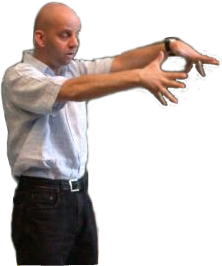
\includegraphics[width=0.7\linewidth]{bilder/dozenten/fekete_frei.png}\\
\textit{Prof. S\'andor Fekete}

Diese Vorlesung vermittelt Programmiersprachenunabh"angige Konzepte wie B"aume, Listen oder Stacks. Wer nicht wei"s, was sich hinter diesen Begriffen verbirgt, sollte auf keinen Fall die "Ubungen verpassen.

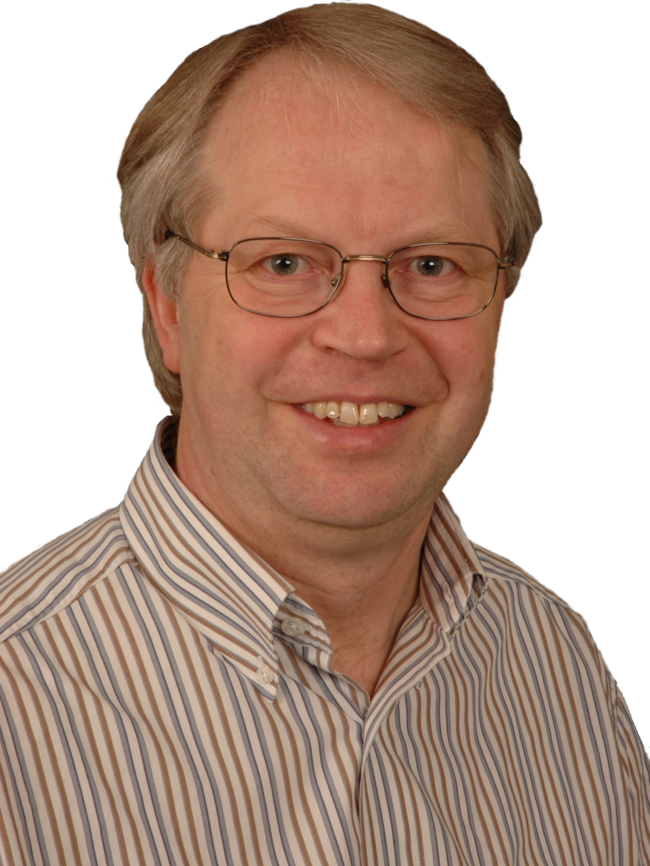
\includegraphics[width=0.6\linewidth]{bilder/dozenten/struck.png}\\
\textit{Dr. Werner Struckmann}

\subsubsection{Programmieren 1}

Programmiert wird hier fast ausschlie"slich in Java. Wer keine oder nur wenig Erfahrungen mit Java gemacht hat, sollte unbedingt die kleinen "Ubungen bearbeiten.
%Die Klausur ist ber"uhmt f"ur ihre hohe Durchfallquote! (Gl"ucklicherweise sind daran nicht die Informatiker schuld)
%Trotzdem: Programmieren ist das Handwerk der Informatik, also macht eurem Fach Ehre.

\subsubsection{Lineare Algebra}


\includegraphics[width=0.8\linewidth]{bilder/dozenten/marten_frei.png}\\
\textit{Dr. Wolfgang Marten}

Hier geht es um Vektoren und Matrizen, sowie ein wenig Gruppentheorie.
Die "Ubungen sind zwar nicht immer einfach, geben aber einen sehr guten Ausblick auf die Klausur.

\subsubsection{Diskrete Mathematik}

% \begin{figure}[h]
% 	\centering\includegraphics[width=0.7\linewidth]{bilder/kemnitz.png}\\
% 	{Dr. Arnfried Kemnitz}
% \end{figure}
Diskrete Mathematik handelt von allem, was mit ganzen Zahlen zu tun hat: Fibbonacci-Zahlen, Primzahlen, Modulorechnung, usw.
Die Veranstaltung wird von Dr. Arnfried Kemnitz gehalten (leider kein Foto).


\subsubsection{Wissenschaftliches Arbeiten}


\includegraphics[width=0.9\linewidth]{bilder/dozenten/jung_frei.png}\\
\textit{Prof. Helmut Jung}

In dem Kurs "`wissenschaftliches Arbeiten"' lernen die Teilnehmer/-innen, Schritt f"ur Schritt eine wissenschaftliche Arbeit durchzuf"uhren -- beispielsweise eine Bachelorarbeit.
Hierzu erfahrt ihr, wie man systematisch vorgeht und welche Methoden man in welchem Schritt verwenden kann.
Die Veranstaltung findet in zwei Gruppen statt, eine bei Prof. Jung und die andere bei Dr. Herrmann.
% Das gehört eigentlich nicht hier hin:

%Die Veranstaltung wird in zwei Gruppen angeboten: Der erste Kurs bei Prof. Jung findet Montag von 9:45 bis 11:15 Uhr und Dienstag von 11:30 bis 14:45 Uhr statt.
%Der zweite Kurs bei Dr. Herrmann findet Dienstag von 15:00 bis 16:30 Uhr statt.
%Beide Kurs haben denselben Inhalt und dieselbe Stundenzahl.
%Der zweite Kurs dauert das gesamte Semester, der andere endet entsprechend fr"uher.

\subsection{Interview mit PD Dr. Bode}

Privatdozent Dr. Bode leitet die großen und kleinen Übungen zur
Vorlesung ,,Diskrete Mathematik für Informatiker''. Er hat sich
freundlicherweise für ein Interview zur Verfügung gestellt.

\nquestion{Was und wo haben Sie studiert?} \\
Ich habe hier an der Technischen Universität Mathematik mit Nebenfach
Informatik studiert. Neben dem Diplom in Mathe habe ich dazu noch das
Vordiplom in Informatik gemacht.
\nquestion{Welchen Bezug haben Sie als Mathematiker zu Informatik?}\\
Für mich sind Computer in erster Linie ein Werkzeug, um bestimmte
mathematische Probleme zu lösen. Im Studium habe ich dazu
hauptsächlich Vorlesungen aus der theoretischen Informatik
gehört. Daneben habe ich als studentische Hilfskraft die Vorlesungen
,,Theoretische Informatik 1/2'' betreut.
%\nquestion{Erzählen Sie eine kleine Anekdote aus Ihrem Studium!}\\
\nquestion{Worum geht es in der Veranstaltung ,,Diskrete Mathematik für
Informatiker''?}\\
Sie behandelt wichtige Grundlagen, die die Studierenden später
brauchen werden. Inhaltlich geht es zunächst um allgemeine Grundlagen,
bevor wir uns etwas Kombinatorik, Zahlentheorie und Algebra angucken. \\
\nquestion{Welche Rolle spielen dabei die Übungen?}\\
Nun, die Übungen sind eine Ergänzung zur Vorlesung, die beim
Verständnis helfen sollen. Dazu sind sie eine gute Vorbereitung für
die Klausur. Dies klappt aber nur bei aktiver Mitarbeit der
Studierenden. Man sollte sich die Aufgaben schon vorher mal angeguckt
haben, sonst bringt das nichts. \footnote{Anmerkung des Interviewers:
Das kann ich aus eigener Erfahrung bestätigen, auch wenn man dabei
noch nichts versteht :)}. Die Meisten verhalten sich leider am Anfang
sehr passiv.\\
\nquestion{Was können Sie den Studierenden für das erste Semester mit
auf den Weg geben?}\\
Sie sollten  nicht alles glauben, was man ihnen
erzählt. Letztes Jahr gab es das Gerücht, dass die 1. große Übung
ausfällt, da es ja noch keine Vorlesung gab. Dem war nicht so, wir
haben da die Übungseinteilung gemacht. Da weniger anwesend waren, gab
es am Ende nicht so viele Übungen, wie man eigentlich gebraucht
hätte. Im Zweifelsfall gilt die Webseite zur Übung
\nurl{http://www.mathematik.tu-bs.de/jpbode/dm/}. Dort werden auch die
Übungsblätter veröffentlich.\\
Neben diesen speziellen Ratschlag noch einen Allgemeinen: Niemand wird
dafür umgebracht, Fragen zu stellen. Wenn also etwas unklar ist, nur
Mut!\\
\nquestion{Vielen Dank für das Interview!}\\
Bitte sehr. Zum Abschluss möchte ich allen Erstsemestern noch viel
Spaß und Erfolg im Studium wünschen.

\newpage
\subsection*{\Large{Du bist computers"uchtig, wenn\ldots}}

\begin{enumerate}
\item \ldots du eine Viertelstunde brauchst, um durch deine Bookmarks zu scrollen.
\item \ldots du deinen Lautsprecher aufdrehst, bevor du das Zimmer verl"a"st, damit du das akustische Signal h"orst, wenn eine neue E-Mail eintrifft.
\item \ldots dein Hund eine eigene Homepage hat.
\item \ldots du deine Mutter nicht anrufen kannst, weil sie kein VoIP-Telefon hat.
\item \ldots du deine Mail abrufst, die Meldung kommt: "`No new messages"' - und du sie gleich nochmal abrufst.
\item \ldots du das Geschlecht von dreien deiner besten Freunde nicht kennst, weil sie neutrale Nicknames haben und du sie nie danach gefragt hast.
\item \ldots du morgens um 3 Uhr aufwachst, zum Klo gehst und auf dem R"uckweg am Computer halt machst, um deine Mailbox abzurufen.
\item \ldots du dich t"atowieren l"asst: "`Diesen K"orper betrachtet man am besten mit Mozilla 5.0 oder h"oher"'.
\item \ldots dein Partner sagt, dass das Gespr"ach f"ur eine Beziehung wichtig ist, also kaufst du einen zweiten Rechner und richtest ihm/ihr einen IRC-Client ein.
\item \ldots dir jemand einen Witz erz"ahlt und du mit *lol* antwortest.
\item \ldots du deinen Freunden von einer hei"sen Verabredung erz"ahlst und ihnen verschweigst, dass sie in einem Chatroom stattfindet.
\item \ldots du dir einen Laptop kaufst, um auch auf dem Klo surfen zu k"onnen.
\item \ldots du auf eine Webseite schaust, die voll mit Links von jemand anderem ist, und alle Links bereits in Lila erscheinen.
\item \ldots dich dein Provider bei technischen Schwierigkeiten um deine Hilfe bittet.
\item \ldots du bei \nurl{http://www.wetter.de/} nachschaust, anstatt aus dem Fenster.
\item \ldots Google bei dir anfragt, was noch in ihrer Suchmaschine fehlt.
\item \ldots du deinen Kopf zur Seite beugst, um zu l"acheln.
\item \ldots deine Kaffeemaschine eine eigene IP hat.
\item \ldots du versuchst Texte aus deinem handgeschriebenen Script per copy and paste in ein \LaTeX-Dokument einzuf"ugen.
\item \ldots du keine Kiste mit alten Computerteilen hast, weil z.B. der alte 386er noch als Anrufbeantorter genutzt wird.
\item \ldots du deine HiFi-Anlage "uber einen eigens daf"ur aufgesetzten Webserver steuerst.
\item \ldots du bei vier Webbrowserspielen unangefochten auf Platz 1 stehst.
\item \ldots du wei"st, was man unter\\ \nurl{http://www.google.de/search?&amp;q=5\%5E2\%2B23\%2D3\%21&amp;btnG=Suche&amp;meta=} findet.
\end{enumerate}

  \section{Was du tun solltest}
% !TEX root = ../../1-te.tex

\subsection{Checkliste}
\label{checkliste}
	Hier wird zusammengefasst, was du in den ersten Tagen des Studiums unbedingt erledigen solltest. Wenn du die ToDos auf der Checkliste nach Erledigung abhakst, verlierst du nicht den Überblick und vergisst nichts.
	
\vspace*{0.5cm}
% !TEX root = ../../1-te.tex

\begin{tabular}{|p{3mm}|l|l|c|c|}
\hline \checkmark 
       & \textbf{Todo}             & \textbf{Zu erledigen bis}                                  & \textbf{Seite}               & \textbf{Muss?} \\ 
\hline & BAföG beantragen          & Spätestens Ende \iftoggle{winter}{Oktober}{April}          & \pageref{todobafoeg}         & optional \\ 
\hline & Wohnsitz Ummelden         & 1 Woche nach Umzug                                         & \pageref{todoummelden}       & ja \\ 
\hline & Mailinglisten             & So früh wie möglich                                        & \pageref{mailinglisten}      & ja \\ 
\hline & Studiengrobplanung        & Vor dem Stundenplanbauen                                   & \pageref{grob}               & ja \\ 
\hline & Auflagen klären           & So früh wie möglich, final: Ende 2. Semester               & \pageref{auflagen}           & nur Master \\ 
\hline & Persönlicher Stundenplan  & Siehe Terminzettel der Fachgruppe                          & \pageref{masterstundenplan}  & ja \\ 
\hline & Prüfungsbogen             & Apätestens \iftoggle{winter}{Dezember}{Mai}                & \pageref{todoanmeldung}      & ja \\ 
\hline & Prüfungsanmeldung         & Anmeldewoche (30.05 - 03.06) oder Online (09.05 - 20.06)   & \pageref{todoanmeldung}      & ja \\ 
\hline & Blog abonnieren           & So früh wie möglich                                        & \pageref{fachgruppe}         & ja \\ 
\hline & Prüfungsordnung lesen     & Zu den ersten Klausuren                                    & \pageref{po}                 & ja \\ 
\hline & TUcard validieren         & Zu Beginn und zu jedem neuen Semester                      & \pageref{tucard}             & ja \\
\hline & Bibliotheksausweis        & Vor der ersten Buchausleihe                                & \pageref{todobib}            & optional \\
\hline & Kopierkarte               & Wenn man was kopieren muss                                 & \pageref{todobib}            & optional \\ 
\hline
\end{tabular} 
\tocheck{2}{Exakte Daten Anmeldewoche einfügen, s.\url{https://www.tu-braunschweig.de/fk1/service/informatik/pa/}}

\begin{multicols}{2}

\subsubsection{BAföG}
	\label{todobafoeg}

	Wer BAföG beantragen möchte, sollte sich am besten gründlich informieren. Sehr zu empfehlen ist da: \\
	\verUrl{2}{http://www.bafoeg.bmbf.de/}
 
	Förderungsanträge gibt es zum Download oder in Papierform im EG des BAföG-Amtes, Wilhelmstraße 1. Wenn du BAföG beantragen möchtest, stelle den Antrag so früh wie möglich, denn es wird nicht rückwirkend gezahlt.

	Zum Anfang des Semester ist mit längeren Wartezeiten zu rechnen, im Notfall kannst du beim AStA-Sozialreferat ein kurzfristiges, zinsloses Darlehen beantragen, um den ersten Monat zu überbrücken. Das Darlehen ist auf 350 Euro begrenzt und muss innerhalb von vier Monaten zurückgezahlt werden. Mehr Informationen findest du auf der Seite des Sozialreferats: \verUrl{2}{https://www.asta.tu-braunschweig.de/de/referate/sozialreferat/}


\subsubsection{Ummelden}
	\label{todoummelden}

	Wer neu nach Braunschweig gezogen ist, muss sich innerhalb einer Woche beim Einwohnermeldeamt anmelden. Wenn ihr die Frist verpasst, drohen theoretisch Strafen, aber praktisch sieht es da nicht so streng aus. Wenn man Braunschweig als Erstwohnsitz wählt, bekommt man (ein Jahr später) eine einmalige Zuzugsprämie von 200 Euro (Immatrikulationsbescheinigung nicht vergessen). Alternativ kann man Braunschweig auch als Zweitwohnsitz wählen.

\subsubsection{Prüfungsanmeldung}
	\label{todoanmeldung}

	Du musst dich für alle Prüfungen, an denen du teilnehmen willst, vorher beim Prüfungsamt anmelden. Die Fristen sind relativ früh im Semester. Die Termine werden im Laufe des Semesters veröffentlicht (Seiten des P-Amtes (\verUrl{2}{https://www.tu-braunschweig.de/fk1/service/informatik/pa}), Mailingliste). Prüfungen können während der Prüfungsanmeldungswoche schriftlich im Prüfungsamt angemeldet werden oder online über das QIS-Portal. Die Onlineanmeldung ist meist länger als eine Woche freigeschaltet.
	Vor deiner ersten Prüfungsanmeldung musst du außerdem ein Datenblatt ausfüllen. Es empfiehlt sich, das bereits vor der Anmeldewoche zu machen, weil die Schlangen dann nicht so lang sind.

	Für die Online-Anmeldung benötigst du eine TAN-Liste, die du dir vorher im Prüfungsamt organisieren musst.

	Unter folgendem Link findet ihr außerdem alle Prüfungstermine für die Informatik: 
	\verUrl{2}{https://www.tu-braunschweig.de/fk1/service/informatik/pa/}

\subsubsection{TUcard}
	\label{tucard}
	
	Der neue elektronische Studierendenausweis TUcard ersetzt das Leporello, das bislang den Studentenausweis, die Immatrikulationsbescheinigung, Wahlabschnitte und vieles mehr enthielt. Darüber hinaus kannst du deine TUcard als Bibliotheksausweis und Mensakarte nutzen.

	Damit die Karte gültig ist, muss sie zu Beginn und zu jedem neuen Semester validiert werden. Das bedeutet, dass der Thermostreifen auf der Karte in einem Validierungsdrucker mit den aktuellen Daten beschrieben wird.

	Das Börsenguthaben der Karte, beispielsweise zum Bezahlen in der Mensa, kann an Börsenaufwertern (auch denen, die sich bereits in den Mensen befinden) aufgeladen werden.

	Zum Drucken kann Guthaben der Karte auf ein Druckkonto umgebucht werden. Dies geschieht an den Druckkontenumbuchern.

	Weitere Informationen zur TUcard findet ihr unter: \verUrl{1}{https://www.tu-braunschweig.de/studium/imstudium/tucard}

\subsubsection{Uni-Bibliothek}
	\label{todobib}

	Um Bücher in der Uni-Bibliothek ausleihen zu können, brauchst du einen Ausweis. Dieser ist in deiner TUcard integriert. Diesen kannst du an einem der Terminals in der Bibliothek, oder online beantragen und am Schalter freischalten. Je nachdem, ob du zu Beginn schon Bücher brauchst, kannst du die Karte auch später aktivieren.

	In der Bibliothek stehen außerdem Kopierer bereit, die ihr nutzen könnt. Einen davon könnt ihr mit Kleingeld befüllen, kompfortabler geht es aber mit einer Kopierkarte. Die bekommt ihr für ein paar Euro direkt in der Bibliothek. Zu Semesterbeginn gibt es oft noch Einführungskurse in die Bibliotheksbenutzung. Ob ihr euren Bibliotheksausweis vor oder nach diesem Kurs aktiviert, ist egal.
	
\end{multicols}

\subsection{Sonstige Informationen}
\subsubsection{Sprachenzentrum}
Am Sprachenzentrum der Uni kannst du verschiedene Sprachkurse belegen, die du auch als Schl"usselqualifikationen in deinen Bachelor-Abschluss einbringen kannst.
Auf den Seiten des Sprachenzentrums (\nurl{www.sz.tu-bs.de}) findest du alle angebotenen Kurse.
Um sich f"ur Kurse anzumelden, brauchst du ein Konto, das du pers"onlich in der Mediothek (im Altgeb"aude \nurl{http://www.sz.tu-bs.de/mediothek/}) registrieren musst.
\textbf{Wichtig!} Die Anmeldung f"ur Sprachkurse beginnt bereits vor jedem Semester.
Um Pl"atze zu bekommen, solltest du dich also so fruh wie moglich anmelden.
Bevor du an einem Englischkurs teilnehmen kannst, musst du zun�chst einen Einstufungstest machen.
Die Termine findest du hier: \nurl{http://www.sz.tu-bs.de/cn/fremdsprachen/englisch/einstufungstest/}
Da gerade bei diesen Kursen die Nachfrage sehr hoch ist, solltest du den Test m"oglichst bereits vor dem Anmeldungszeitraum (beginnt etwa 2 Wochen vor Vorlesungsbeginn) ablegen.

\subsubsection{Schl�sselqualifikationen}
Jeder Bachelorstudent muss sogenannte Schl"usselqualifikationen innerhalb seines Studiums erwerben.
In der Informatik m�ssen dies "`handlungsorientierte Anwendungen"' im Umfang von 10 Leistungspunkten sein.
Hierzu z"ahlen Sprachkurse und �berfachliche Lehrveranstaltungen.
Informationen "uber das aktuelle Angebot (Pool-Modell) und die zu erf"ullenden Bestimmungen der Veranstaltungen findet ihr auf dieser Webseite: \nurl{http://www.tu-braunschweig.de/informatik-bsc/struktur/schluessel}

\newpage

\subsubsection{Auslandsaufenthalt}
"Uber Auslandssemester solltest du dich ebenfalls so fr"uh wie m"oglich mit dem "`International Office"' (\nurl{http://tu-braunschweig.de/international}) unterhalten.
Der n"achste Termin f"ur die Infoveranstaltungen "`Wege ins Ausland"' und "`Studieren in Europa"' ist der 05.11. ab 16 Uhr im International Office (BW 74). 
  %\begin{multicols}{2}
	\subsection{Wozu Computer?}
		\subsubsection{Vorlesungen Online}
			Zu den meisten Vorlesungen kann man die Skripte im Internet finden. Für einige Vorlesungen gibt es sogar Ton- oder Videomitschnitte.

			Es gibt auch immer engagierte Studierende, die ihre Vorlesungsmitschriften online stellen. Da diese sehr wahrscheinlich in deinem Semester sind, hilft es, wenn du dich in den Vorlesungen umhörst. Ansonsten ist \url{https://www.clevershit.de} die richtige Anlaufstelle für den Informationsaustausch zwischen Studenten.

		\subsubsection{Organisatorisches ohne Papier}
			Ansonsten gibt es eine Reihe von Informationen, die man nur über das Web bekommt, und mehr und mehr Formalitäten (z.B. die Prüfungsanmeldung) werden auch in die virtuelle Relatität verlagert.

			Desweiteren kannst du dir im Netz einen individuellen Stundenplan zusammenstellen, in Erfahrung bringen, wann die nächsten Klausuren stattfinden, lesen, was es in der Mensa zu essen gibt, endlich herausfinden, wann das Prüfungsamt geöffnet hat,  offene HiWi"~Stellen bei den Instituten finden und vieles mehr.

			Die Webseiten der TU sind ein großer Dschungel, durch den man sich am besten  mit Machete und Googlesuche kämpft. Um an der TU etwas zu finden, solltest du deinem eigentlichen Suchbegriff wahlweise \enquote{tu braunschweig} oder \enquote{site:tu-braunschweig.de} anhängen, und schon hast du gute Chancen zum Ziel zu kommen.

		\subsubsection{Mitschreiben am PC}
			Auf den ersten Blick mag es naheliegen, sich
			während der Vorlesungen Notizen  am Laptop
			anzufertigen. In der Praxis gibt es da aber eine
			Reihe von Problemen, vor denen wir  warnen
			möchten. Es hat schließlich seinen Grund, das
			nur 10\% der Studenten in der Vorlesung am
			Laptop sitzen und davon 90\% diesen nur nutzen,
			um zu zocken: Die meisten Tafelanschriften
			bestehen  aus verschachtelten Formeln,
			fremdartigen Buchstaben und verworrenen
			Zeichnungen. Diese in Echtzeit in den Laptop
			einzuhacken ist eine besondere Kunst, die du mit
			Notepad und Word gar nicht erst probieren
			brauchst. Eine Chance hast du vielleicht mit
			einem Tablet PC, oder wenn du
			\LaTeX\ bereits im Schlaf beherrscht -
			aber wer tut das schon zu Beginn des Studiums?

			In den Vorlesungen, in denen du nicht Tafelweise abschreiben musst, sondern nur hier und da mal etwas notieren, zeigt sich der PC schon als nützlicher. Wenn du ab und zu den Vortrag des Profs damit vergleichen möchtest, was er in sein Skript geschrieben hat, kann dir der mitgebrachte Laptop unter Umständen das Ausdrucken von ein paar hundert Seiten ersparen. Du wirst aber schnell merken, dass es in praktisch keinem der Hörsääle und Seminarräume Steckdosen gibt, und in manchen nichtmals ausreichende WLAN-Signalstärke.

		\subsubsection{Hausaufgaben am PC}
			In vielen Fächern musst du regelmäßig
			Hausaufgaben erledigen und einreichen. Keiner
			erwartet von dir, dass diese mit dem PC gemacht
			werden, es ist also völlig ok sie von Hand zu
			schreiben. Es hat aber auch gewisse Vorteile,
			sie am PC zu schreiben (z.B. mittels \LaTeX) und
			dann auszudrucken. Bei \LaTeX\ handelt es sich
			um ein Satzsystem für wissenschaftliche
			Texte wie Haus- oder Abschlussarbeiten.
			Erwähnenstwert ist die hervorragende
			Unterstützung für den Satz mathematischer
			Formeln und dass dabei mit Befehlen, ähnlich wie
			in HTML gearbeitet wird. Es gibt \LaTeX-Kurse die du im Schlüsselqualifiktationsbereich anrechnen lassen kannst, aber mit den Infos im WWW kann man sich das auch selbst beibringen. Je eher du damit anfängst, desto weniger Probleme hast du später, wenn du damit z.B. deine Abschlussarbeit aufsetzt.

		\subsection{Computer-Pools an der Uni}
			Es ist immer nützlich zu wissen, wo man mal schnell an einen Computer kann. Zumindest ab und zu wirst du die Computer in der Uni benutzen, besonders die Linuxarbeitsplätze in \textbf{PK4.5} oder \textbf{PK4.8}, an denen du die Hausaufgaben für Programmieren abgeben musst.

			\begin{itemize}
				\item[*] Im Erdgeschoss des Altbaus gibt es auf der rechten Seite zwei Computerräume, einen weiter vorne (\textbf{PK4.6}) und einen genau in der Ecke des Gebäudes (\textbf{PK4.5}). Zwei weitere Räume (\textbf{PK4.8} und die \textbf{Datenstation}) findest du im ersten Stock des Altbaus, auch wieder in der rechten Ecke. Die Rechner in \textbf{PK4.5} und \textbf{PK4.8} sind mit Linux ausgestattet. Im ersten Stock gibt es nun auch einen Windowsrechnerraum. Da kann man mal eine Word- oder Powerpoint-Datei ausdrucken, wenn man denn muss.

				\item[*] Reichlich Computer findet man schließlich im Gauß-IT-Zentrum~(GITZ) an der Hans-Sommer-Straße. Das ist der gedrungene, fast würfelförmige, dunkle Klotz hinter dem Elektrotechnik-Hochhaus (\emph{E-Tower}). Hier gibt es mehrere frei zugängliche Räume mit  Linux- und Windowsrechnern. Es gibt hier auch Räume für Medienbearbeitung, wo du etwa Video-Digitalisierer, ein Tonstudio und Rechner mit der Adobe Creative Suite Production Premium nutzen kannst.

				\item[*] Seit 2010 stellt das IBR (Institut für Betriebssysteme und Rechnerverbund) im Raum G40 des Informatikzentrums einen Rechnerraum mit vielen, schnellen Linux-Rechnern  zur Verfügung. Zu diesem CIP-Pool (Computer-Investitions-Programm) bekommt man mit seiner y-Nummer Zutritt. Wenn man Glück hat, funktioniert sogar einer der beiden Drucker in diesem Raum, so dass man zum Drucken nicht das IZ verlassen muss.
			\end{itemize}

		\subsection{Der eigene Rechner}
			Wenn du trotz aller Widrigkeiten planst, dir
			extra für's Studium einen (tragbaren) Rechner
			anzuschaffen, dann hast du hier gleich ein wenig
			Kaufberatung: Viel (Rechen- bzw.
			Grafik-)Leistung brauchst du im Studium  nur für
			sehr wenige spezielle Fachgebiete - das
			einfachste Netbook wird also vermutlich schon
			reichen. Wichtiger ist vielmehr die Akkulaufzeit
			und die WLAN-Empfangsstärke. %a die Här	

		\subsubsection{Welches System?}
			Dir wird auffallen, dass zwar alle Systeme geduldet sind, aber die Linux hier deutlich öfter über den Weg laufen wird als in der freien Wildbahn. Auch wir sind große Linux-Fans und haben deshalb ab Seite \pageref{linux} ein paar Infos dazu zusammengetragen.

			Aber trotz dieser nicht ganz unauffälligen Beeinflussung gilt: Beim Betriebssystem hast du freie Wahl. Sämtliche Software, die du für's Studium brauchen  könntest, gibt es für alle großen Systeme, meist sogar gratis. Für Linux ist eh  praktisch alles frei erhältlich, für Windows spendiert Microsoft den Studenten auch alles außer Office (siehe Seite \pageref{msdnaa}), und auch Apple bringt dich dank satter Studentenrabatte durch Bachelor und Master. 

		\subsubsection{Wege ins Uni-Netz}
			Um den eigenen Rechner ins Netz zu bekommen, stehen die in der Uni WLAN und LAN offen. Zur Konfiguration siehe Seite \pageref{wlan}.

			Für manche Aktivitäten (z.B. den Zugriff auf Prüfungsprotokolle) musst du dich direkt im Uni-Netz befinden. Wenn du und dein Rechner aber gerade zuhause oder sonstwo sind, heißt dass nicht, dass du dich nun physisch auf den Weg machen musst. Mittels VPN kannst du dich virtuell ins Uni-Netz einklinken. Schau einfach mal auf den Seiten des GITZ nach, um mehr zu erfahren.
%\end{multicols}

  \section{Freizeit}
\begin{figure*}[b]
	\centering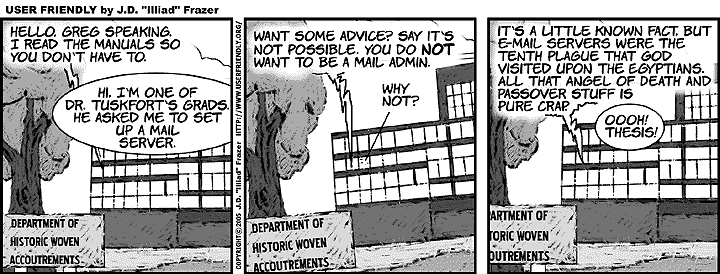
\includegraphics[width=\textwidth]{bilder/comics/uf008003.png}
\end{figure*}
\subsection{Discos}

\begin{description}
\item[Ballhaus] \hfill K"uchenstra"se 1\\
Do -- Sa \hfill 22 -- 4 Uhr\\
Charts, Tanz

\item[Bogey's] \hfill Stecherstra"se\\
Do -- Sa \hfill ab 21 Uhr\\
Deutschrock, Pop, Schlager

\item[Brain Klub] \hfill Bruchtorwall\\
Do -- Sa \hfill ab 23 Uhr\\
Alternative, Funk, HipHop, Independent, Reggae, Soul, Live-Konzerte und DJ-Shows\\
\nurl{http://www.brain-bs.de}

\item[Jolly Joker] \hfill Broitzemer Stra"se 220\\
Di, Fr \& Sa \hfill 22 -- 4.30 Uhr\\
Alternative, Black Music, Charts, RnB, House, Rock. Vier R"aume, Cocktailbar\\
\nurl{http://www.jolly-joker.de}

\item[Meier Music Hall] \hfill Schmalbachstra"se 2\\
Fr \& Sa \hfill 22 -- 5 Uhr\\
Charts, Independent, Pop, Rock\\
\nurl{http://www.meier-music-hall.de}

\item[Merz] \hfill Gieselerstra"se 35\\
Do -- Sa \hfill ab 21 Uhr\\
Alternative, Pop\\
\nurl{http://www.merz-bs.de}

\item[Schwanensee] \hfill Gieselerstra"se 35\\
Fr \& Sa \hfill 23 -- 4 Uhr\\
Classics, House, Soul

\item[Vibe] \hfill Gieselerstra"se 35\\
Fr \& Sa \hfill 21 -- 3 Uhr\\
Black Music, Funk, Soul\\
\nurl{http://www.vibe-bs.de}

\end{description}


\subsection{Kneipen}

\begin{description}

\item[1/4 Nach] \hfill B"ultenweg 89\\
Bietet die M"oglichkeit zum Bier auch noch eine Runde Billiard zu genie"sen.
Campusviertel\\
\nurl{http://www.viertelnach.de}\footnote{Bei Drucklegung hatte die Seite keine Inhalte, aber vielleicht kommt sie ja wieder\ldots}

% Out of Buisness afik ):
%\item[Anno 1826] \hfill Schleinitzstra"se 1

\item[Charly's Tiger] \hfill Wilhelm-Bode-Stra"se 26\\
Jeden Montag alle Men"us zum halben Preis. Sehr empfehlenswert.


\item[Eusebia] \hfill Spielmannstra"se 11\\
Mischung aus Restaurant, Cafe und Kneipe. Zu jeder Tageszeit empfehlenswert.
Campusviertel

\item[Expertise] \hfill Steinbrecherstra"se 31\\
Gem"utliche Spielekneipe mit einer riesigen Auswahl an Brettspielen.

\item[Funzel] \hfill Rebenring 9\\
  %Neue adresse nachgucken!
Hat meistens ziemlich lange auf. Wer es urig mag, wird hier gl"ucklich.
Campusviertel

\item[Herman's Cafe Bar] \hfill Schleinitzstra"se 18\\
Hier gibt es sehr gute Baguettes, die man in angenehmer Atmosph"are genie"sen kann.
Campusviertel\\
\nurl{www.hermans-cafe.de}

\item[Mephisto] \hfill Fallersleber Stra"se 35\\
Gro"se, aber gem"utliche Kneipe.

%\item[Merz, Vibe, Schwanensee] \hfill Gieselerstr. 35\\
%Alle drei mit unterschiedlicher Musik. Gut zum Rocken geeignet.\\
%\nurl{http://www.merz-bs.de}

\item[Michaelishof]~ \hfill Güldenstr. 8a\\
  Kneipe im Wohnheim Michaelishof\\
  Geöffnet: Donnerstags ab 21:00 Uhr\\
  \nurl{http://www.michaelishof.de/kneipe/}
\item[MonkeyIsland]~ \hfill Rebenring 64\\
  Kneipe im Wohnheim Affenfelsen\\
  Regelmäßig wechselndes ,,Bier der Woche'' und eine riesige
  Spielesammlung\\
  Geöffnet: Donnerstags ab 20:00 Uhr\\
  \\\nurl{http://gruppen.tu-bs.de/monkeyisland/}
\item[R.P. McMurphy's Irish Pub] \hfill B"ultenweg 10\\
Gem"utlicher Irish Pub in Sichtweite der Uni.
Campusviertel
 \item[Schunterkino] \small{Bienroder Weg 54}\\
   \normalsize
   Kinoim Wohnheim an der Schunter\\
   Das Kino verfügt über einen echten Projektor und gemützliche
   Bestuhlung.\\
 %Die Kneipe hat neben    günstigen Preisen zwei Kicker, Tischtennis, Dart und einen
  % Billiardtisch zu bieten.\\
   %Viermal im Jahr werden größere Partys veranstaltet.\\
%   Gemützlicher Kinosaal mit  professionelle Technik bei sehr günstigen
%   Eintritt, regelmäßige Themenabende/Konzerte in der Kneipe, viermal im Jahr
%   größere Partys\\
   Kinovorstellungen: Im Semester Dienstags und Donnerstags ab 20:00 Uhr\\
  % Geöffnet: Dienstags, Donnerstags und Freitags ab 20:00 Uhr
   \\\nurl{http://www.schunterkino.de/}\\
 %  \nurl{http://www.schuntille.de/}
 \item[Schuntille] \small{Bienroder Weg 54}\\
   \normalsize
 Die    Kneipe im Wohnheim an der Schunter 
  % Das Kino verfügt über einen echten Projektor und gemützliche
  % Bestuhlung.\\
  hat neben    günstigen Preisen zwei Kicker, Tischtennis, Dart und einen
   Billiardtisch zu bieten.\\
   Viermal im Jahr werden größere Partys veranstaltet.\\
%   Gemützlicher Kinosaal mit  professionelle Technik bei sehr günstigen
%   Eintritt, regelmäßige Themenabende/Konzerte in der Kneipe, viermal im Jahr
%   größere Partys\\
 %  Kinovorstellungen: Im Semester Dienstags und Donnerstags ab 20:00 Uhr\\
   Geöffnet: Dienstags, Donnerstags und Freitags ab 20:00 Uhr
 %  \\\nurl{http://www.schunterkino.de/}\\
   \nurl{http://www.schuntille.de/}
  % \ \\ \\ \\
   \item[Wild Geese] \hfill G"ordelingerstra"se 49\\
Montags gibt es den Pint f"ur Studenten g"unstiger.
Quizabend und Karaoke.\\
\nurl{http://www.wildgeese.de}

\end{description}
\end{multicols}
%	\end{wrapfigure}
%\newpage
\vfill
\begin{center}
  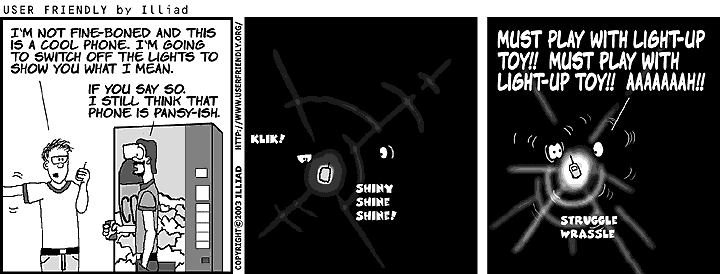
\includegraphics[width=\linewidth]{bilder/comics/uf005633.png}
\end{center}
\newpage
	\begin{multicols}{2}

%%% Local Variables: 
%%% mode: latex
%%% TeX-master: "../../1-te"
%%% End: 

\newpage
\subsection{Tagebücher}
\subsubsection{Tagebuch eines 1. Semesters\ldots}

\begin{description}
\item[05:30] Der Quarz-Uhr-Timer mit Digitalanzeige gibt ein zaghaftes "`Piep-Piep"'
von sich. Bevor sich dieses zu energischem Gezwitscher entwickelt, sofort
ausgemacht, aus dem Bett gehüpft. Fünf Kilometer Jogging an der Oker,
mit einem Besoffenen zusammengestoßen, anschließend eiskalt geduscht.
\item[06:00] Beim Frühstück Heise-Online studiert und dabei neueste Patches geladen.
Danach kritischer Blick in den Spiegel, Outfit genehmigt.
\item[07:00] Zur Uni gehetzt. PK 2.2 erreicht. Pech gehabt: erste Reihe schon besetzt.
Niederschmetternd. Beschlossen, morgen doch noch eher aufzustehen.
\item[07:30] Vorlesung, Algorithmen und Datenstrukturen bei Fekete. Keine Disziplin!
Einige Kommilitonen lesen
Sportteil der BZ oder gehen ins "`Viertel Nach"' frühstücken. Alles
mitgeschrieben. Füller leer, aber über die Witzchen des Dozenten mitgelacht.
\item[08:00] Vorlesung, Lineare Algebra, Marten. Verdammt! Extra neongrünen Pulli
angezogen und trotz eifrigem Fingerschnippens nicht drangekommen.
\item[10:45] Nächste Vorlesung. Nachbar verläßt mit Bemerkung "`Sinnlose
Veranstaltung"' den Raum. Habe mich für ihn beim Prof. entschuldigt.
\item[12:00] Mensa Essen II. Nur unter größten Schwierigkeiten
weitergearbeitet, da in der Mensa zu laut.
\item[12:45] In Fachschaft gewesen. Mathe Skript immer noch nicht fertig. Wollte
mich beim Vorgesetzten beschweren. Keinen Termin bekommen. Daran geht die
Welt zugrunde.
\item[13:00] Fünf Leute aus meiner Stuko-Gruppe getroffen. Gleich für drei AG's zur
Klausurvorbereitung verabredet.
\item[13:30] Dreiviertelstunde im Copyshop gewesen und die Klausuren der letzten 10
Jahre mit Lösungen kopiert. Dann Kleine übung: Ältere Semester haben keine
Ahnung.
\item[15:30] In der Bibliothek mit den anderen gewesen. Durfte aber statt der
dringend benötigen 18 Bücher nur vier mitnehmen.
\item[16:00] Große übung. War gut vorbereitet. Hinterher den Assi über seine
Irrtümer aufgeklärt.
\item[18:30] Anhand einschlägiger Quellen die Promotionsbedingungen eingesehen und
erste Kontakte geknüpft.
\item[19:45] Abendessen. Verabredung im "`Dialog"' abgesagt. Dafür Vorlesungen
der letzten paar Tage nachgearbeitet.
\item[23:00] Videoaufzeichnung von "`Relationale Datenbanken 1"' angesehen und im Bett noch den "`Cormen"'
gelesen. Festgestellt, 18-Stunden-Tag zu kurz. Werde demnächst die Nacht
hinzunehmen.
\end{description}
\begin{center}
  
\includegraphics[width=\linewidth]{bilder/comics/stein1.png}
\end{center}
\newpage
\subsubsection{Tagebuch eines 11. Semesters\ldots}

\begin{description}
\item[10.30] Aufgewacht! Ach, Kopfschmerzen, übelkeit, zu deutsch: KATER!
\item[10.45] Der linke große Zeh wird Freiwilliger bei der Zimmertemperaturprüfung.
(Arrgh!) Zeh zurück. Rechts Wand, links kalt; Mist, bin gefangen.
\item[11.00] Kampf mit dem inneren Schweinehund: Aufstehen oder nicht - das ist
hier die Frage.
\item[11.30] Schweinehund schwer angeschlagen, wende Verzögerungstaktik an und
schalte Fernseher ein (inzwischen auch schon verkabelt).
\item[12.05] Mittagsmagazin beginnt. Originalton Moderator: "`Guten Tag liebe
Zuschauer Guten MORGEN liebe Studenten."' Auf die Provokation hereingefallen
und aufgestanden.
\item[13.30] In der Cafeteria der Mensa Katharienstraße beim Skat mein Mittagessen
verspielt.
\item[14.30] Im Hermanns hereingeschaut. Geld gepumpt und 'ne Kleinigkeit
gegessen: Bier schmeckt wieder! Kurze Diskussion mit ein paar Leuten über
die letzte Entwicklung auf dem Computerspielemarkt.
\item[15.45] Kurz in der Bibliothek gewesen. Nix wie raus, total von Erstsemestern
überfüllt.
\item[16.00] Fünf Minuten im IZ gewesen. Nichts los! Keine Zeitung, keine
Flugblätter\ldots
\item[17.00] Stammkneipe hat immer noch nicht geöffnet.
\item[18.15] Resigniert im fgraum ne Flasche Mate geholt und die neuste bbt folge gesehen.
\item[19.10] Komme zu spät zum Date mit dem blonden Erstsemester im Eusebia.
Immer dieser Streß!
\item[01.00] Die Kneipen schließen auch schon immer früher\ldots Umzug ins Jolly Joker.
\item[04.20] Tagespensum erfüllt. Das Bett lockt.
\item[05.35] Am Okerufer von Erstsemester über'n Haufen gerannt worden. Hat mich
gemein beschimpft.
\item[06.45] Bude mühevoll erreicht. Insgesamt \EUR{27,50} ausgegeben. Mehr hatte der
Kleine nicht dabei.
\item[07.05] Schlucke schnell noch ein paar Alkas und schalte kurz das Radio ein.
Stimme des Sprechers: "`Guten Morgen liebe Zuhörer, gute NACHT liebe
Studenten."'
\end{description}

  \section{N"utzliches}
\begin{multicols}{2}
\subsection{Semesterticket}
	Euer Studentenausweis berechtigt euch zur Fahrt auf vielen Zugstrecken in Niedersachsen. Unten seht ihr den Gültigkeitsbereich des Semestertickets im Großraum Hannover. Nach Norden und und Westen deckt das Semesterticket weitere Strecken ab. Einen grober Überblick gibt die nebenstehende Karte. 

	Es dürfen nur Regionalexpress (RE) und Regionalbahn (RB) der Deutschen Bahn AG, sowie teilweise der Metronom in der zweiten Klasse benutzt werden. Also NICHT Strecken der Nordwestbahn (NWB). Einen genauen Überblick findet ihr in Form einer Streckenliste auf der Seite \pageref{streckenliste1}.

	Mehr Details könnt ihr den Seiten des AStA unter \url{http://www.asta.tu-bs.de/semesterticket.php} bzw. \url{http://tinyurl.com/3gn8fhg} entnehmen.
\end{multicols}
\newpage
%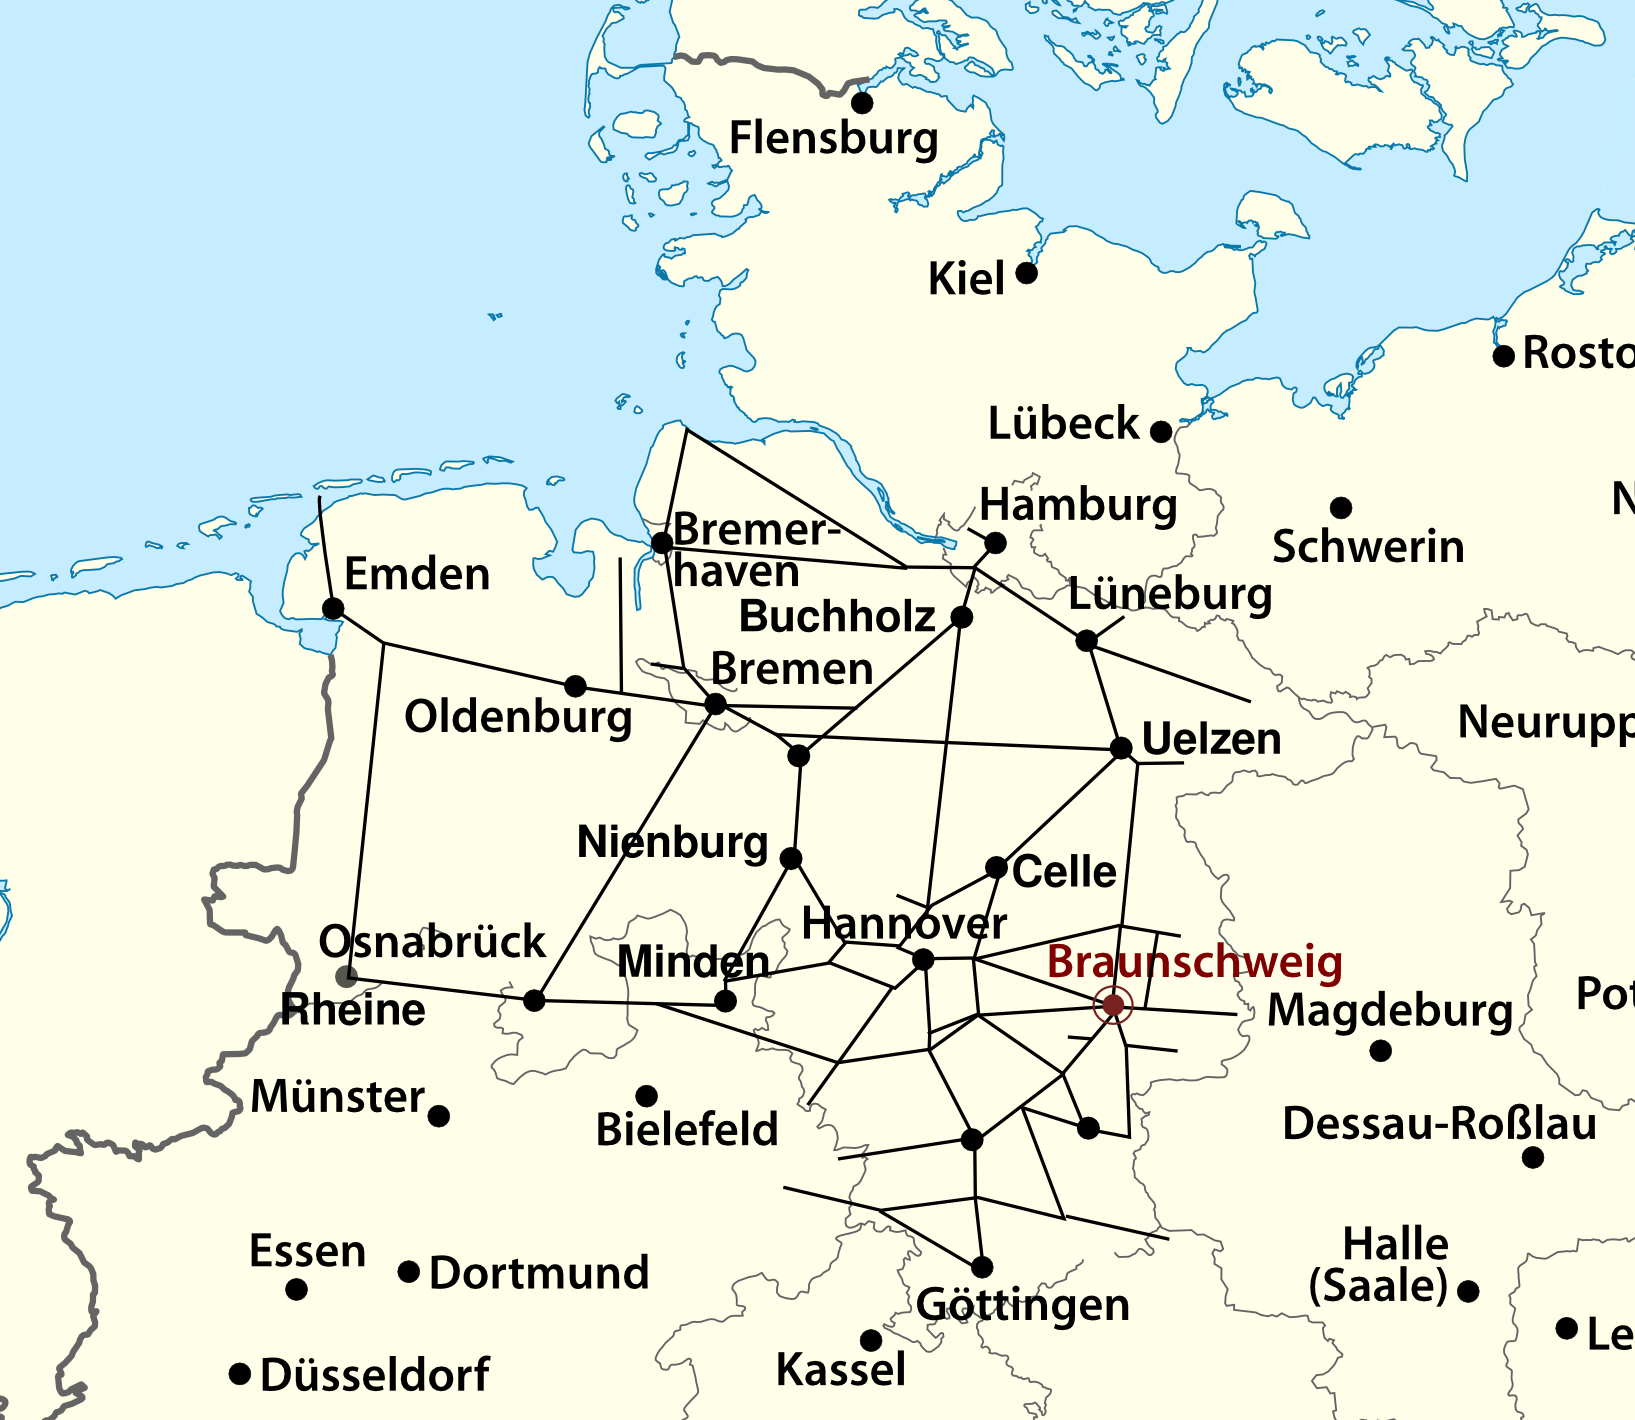
\includegraphics[width=\columnwidth]{bilder/ticket_deutschland.png}
\newpage
%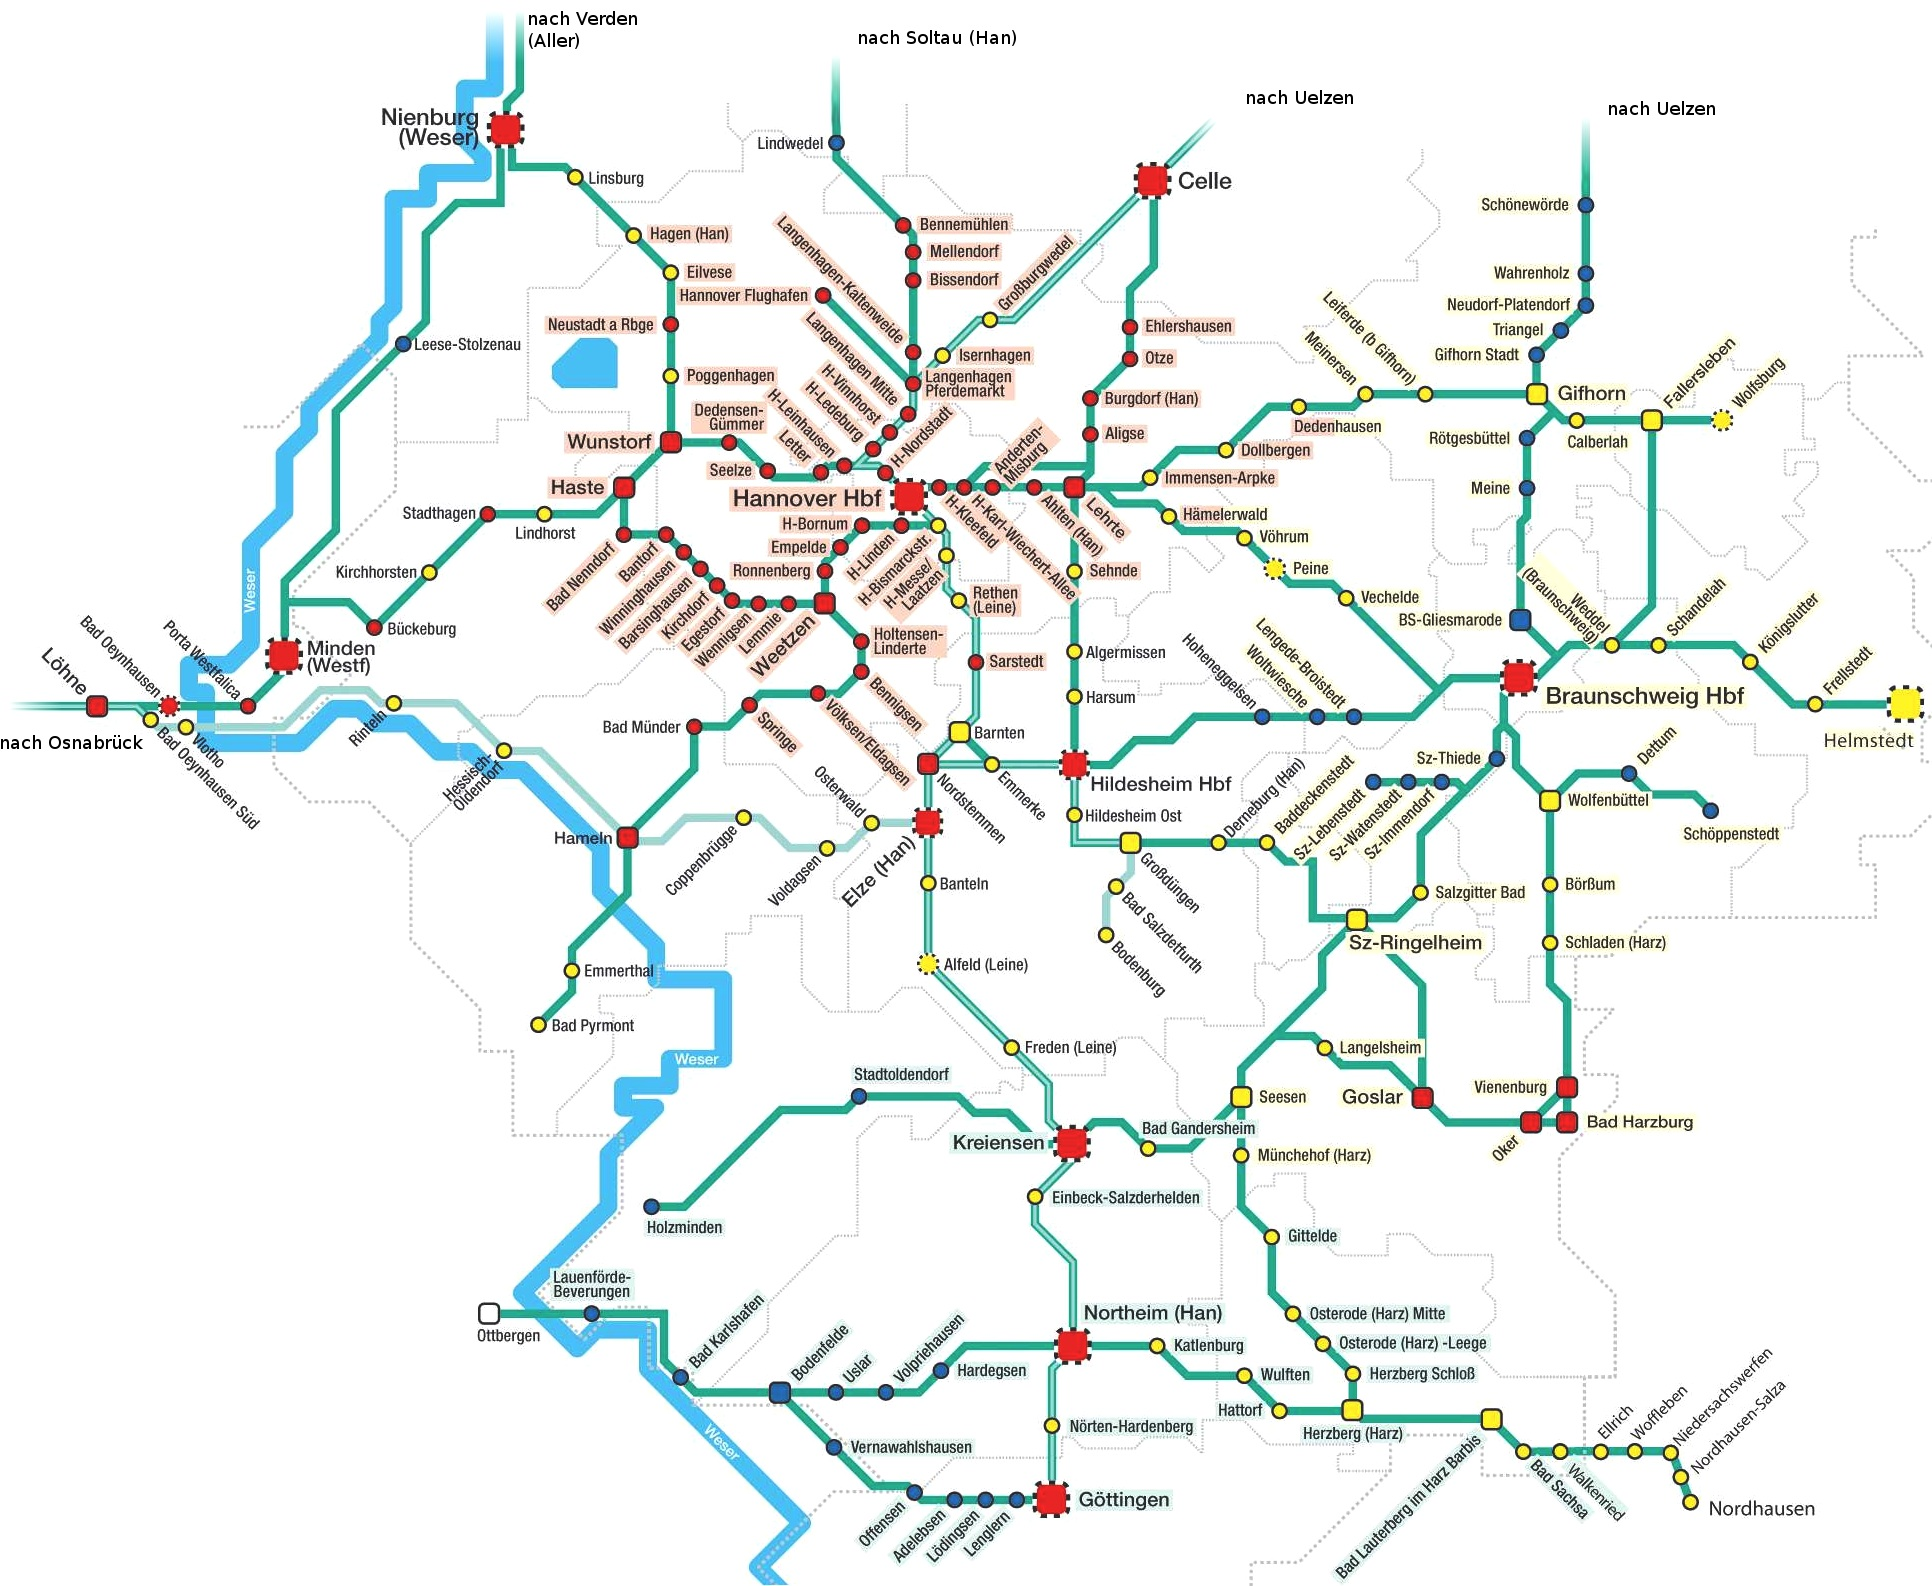
\includegraphics[width=\textwidth]{bilder/ticket_bis_11_Dezember.jpg}
\newpage
\newpage
\begin{multicols}{2}
\subsubsection*{Streckenübersicht Wintersemester 2010/2011 und Sommersemester 2011 gültig ab 1.10.2010}
\label{streckenliste1}
\begin{tabular}{|l|l|l|p{2cm}|}
\hline
\multicolumn{3}{|l|}{\textbf{Strecke/ Streckenabschnitt}}& \textbf{KbN}\\
\textbf{\textit{von}} & \textit{über} & \textbf{\textit{bis}} & \\ \cline{ 1- 4}
Lüneburg &  & Dannenberg Ost & 112 \\ \hline
Braunschweig Hbf & Gifhorn & Uelzen & 115 \\ \hline
Bremen Hbf & Soltau & Uelzen & 116 \\ \hline
Hamburg-Harburg &  & Stade & 121 \\ \hline
Buchholz (Nordheide) & Soltau & Bennemühlen & 123 \\ \hline
Minden Westf. & Nienburg & Rotenburg/Bremen Hbf & 124 \\ \hline
Bremen Hbf &  & Cuxhaven & 125 \footnotemark[1] \\ \hline
Bremen Hbf &  & Bremen-Vegesack & 126 \footnotemark[1] \\ \hline
Echem &  & Lüneburg & 145 \\ \hline
Hannover Hbf & Gifhorn & Wolfsburg Hbf & 300 \\ \hline
Braunschweig Hbf &  & Wolfsburg Hbf & 301 \\ \hline
Uelzen &  & Schnega & 305 \\ \hline
Hannover Hbf & Braunschweig Hbf & Helmstedt & 310 \\ \hline
Braunschweig Hbf & Wolfenbüttel & Schöppenstedt & 312 \footnotemark[2] \\ \hline
Braunschweig Hbf &  & Hildesheim Hbf & 313 \\ \hline
Hannover Hbf & Hildesheim Hbf/Goslar & Bad Harzburg & 320 \\ \hline
Braunschweig Hbf &  & Sz-Lebenstedt & 352 \\ \hline
Braunschweig Hbf & Wolfenbüttel/Vienenburg & Goslar & 353 \\ \hline
Holzminden & Kreiensen & Bad Harzburg & 354 \\ \hline
Ottbergen & Bodenfelde & Göttingen & 356.1 \\ \hline
Ottbergen & Bodenfelde & Northeim & 356.2 \\ \hline
Göttingen & Northeim & Walkenried & 357 \footnotemark[1] \\ \hline
Braunschweig Hbf & Seesen & Herzberg (Harz) & 358 \\ \hline
Haste & Hannover Hbf/Haste & Minden (Westf) & 360.1 \\ \hline
Nienburg (Weser) & Hannover Hbf & Haste & 360.2 \\ \hline
Hannover Hbf & Lehrte & Hildesheim Hbf & 360.3 \\ \hline
Bennemühlen & Hann./Sarstedt & Hildesheim Hbf & 360.4 \\ \hline
Bad Pyrmont & Hameln/Weetzen & Hannover-Flughafen & 360.5 \\ \hline
Celle & Lehrte & Hannover Hbf & 360.6.7 \\ \hline
Hannover Hbf &  & Hannover Bismarckstr. & 361 \footnotemark[1] \\ \hline
Hannover Hbf &  & Löhne (Westf.) & 370 \\ \hline
Löhne (Westf.) & Hameln & Hildesheim Hbf & 372 \\ \hline
Hildesheim Hbf &  & Bodenburg & 373 \\ \hline
Salzbergen & Osnabrück Hbf & Minden (Westf.) & 375 \footnotemark[1] \\ \hline
Bremen Hbf &  & Hannover Hbf & 380 \\ \hline
Osnabrück Hbf &  & Bremen Hbf & 385 \footnotemark[1] \\ \hline
Norddeich Mole & Oldenburg (Oldb) & Bremen Hbf & 390 \footnotemark[1] \\ \hline
Norddeich Mole & Meppen & Rheine & 395 \footnotemark[1] \\ \hline
Emden Hbf &  & Emden Außenhafen & 396 \\ \hline
Leer (Ostfr.) &  & Weener & 397 \\ \hline
\end{tabular}

\footnotetext[1]{nur in den Zügen der DB Regio AG, also nicht in Zügen der Nordwestbahn}
\footnotetext[2]{gültig auch in Bus von  Schöppenstedt-Schöningen-Helmstedt}
\end{multicols}

\subsection{Stundenplan}


\end{document}

